% Created by tikzDevice version 0.9 on 2016-01-12 22:38:50
% !TEX encoding = UTF-8 Unicode
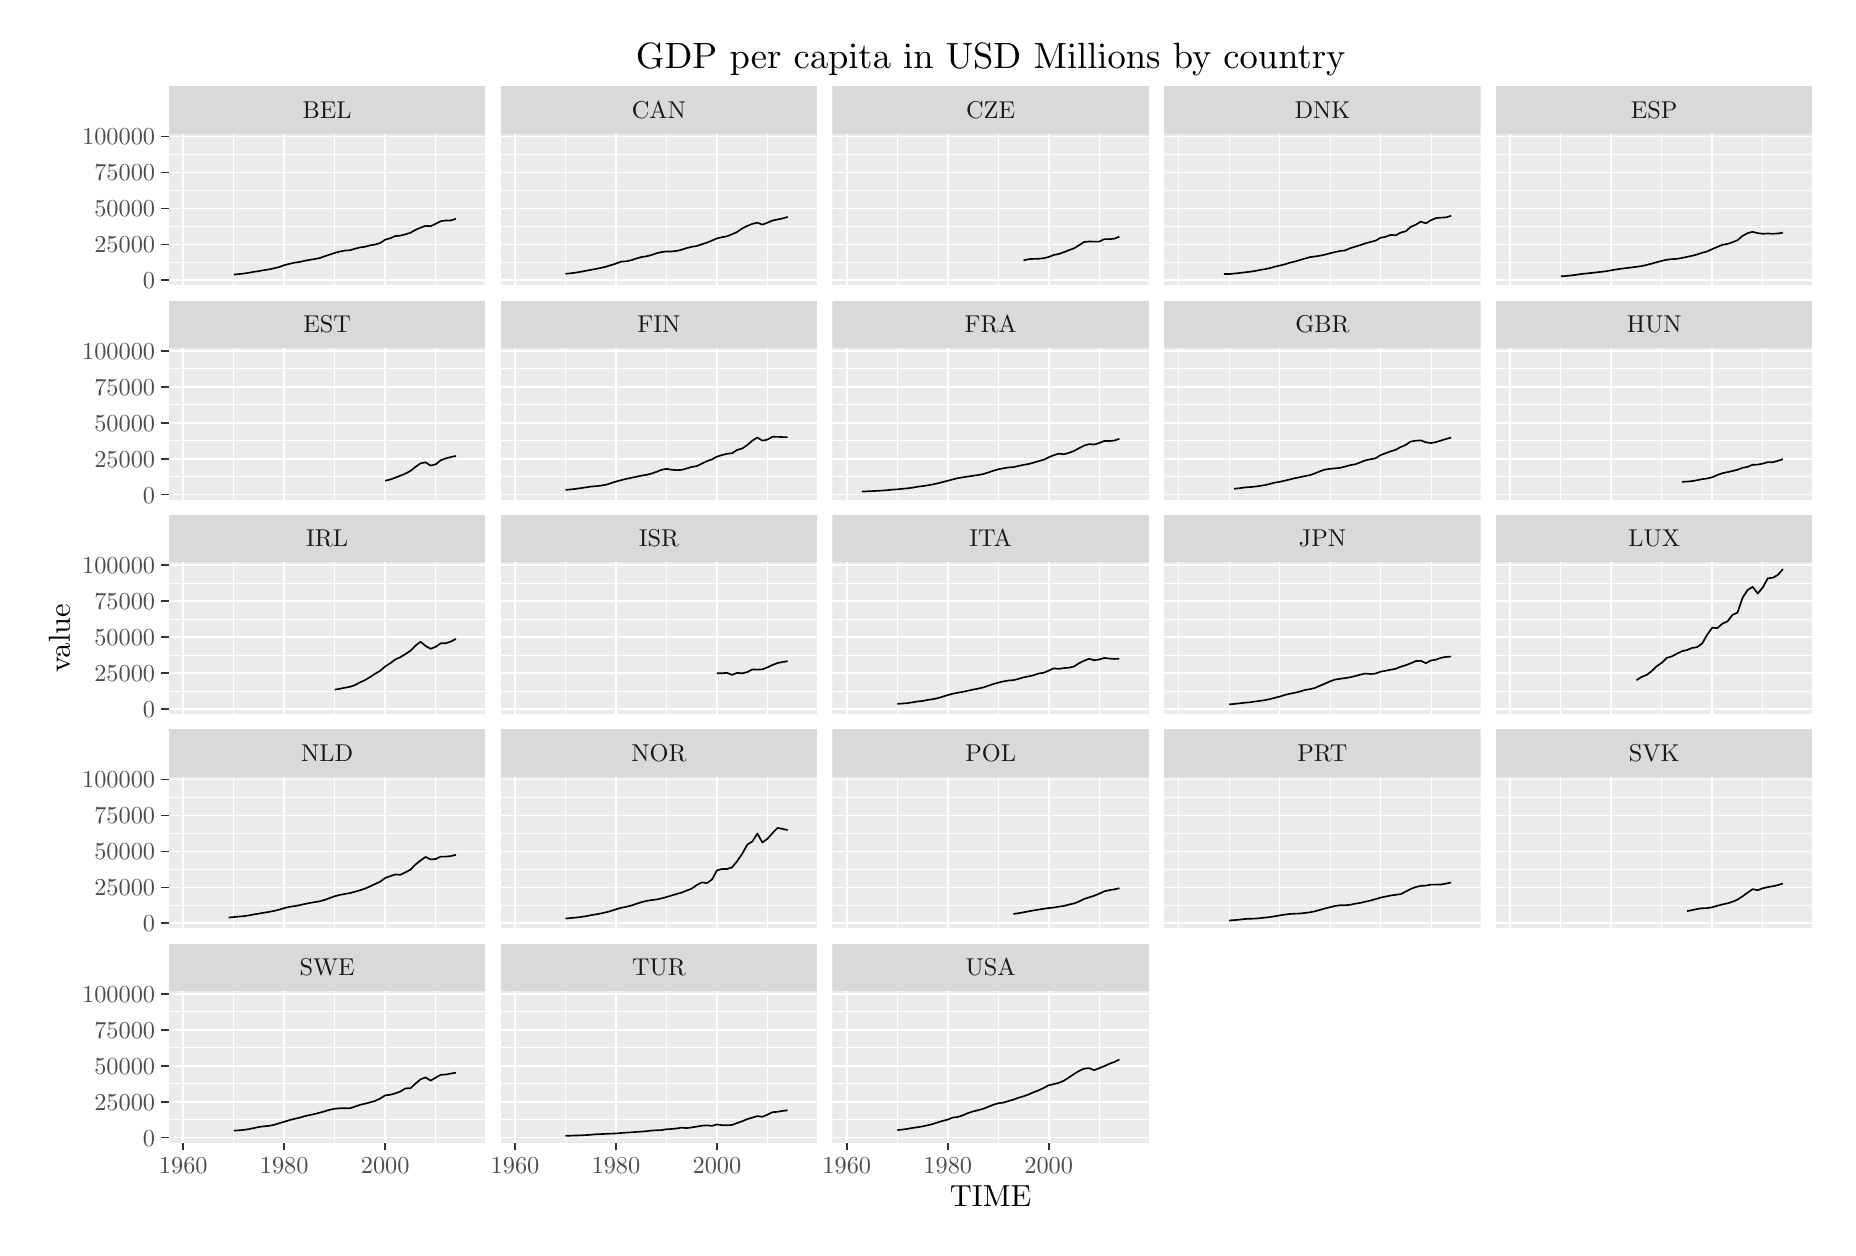
\begin{tikzpicture}[x=1pt,y=1pt]
\definecolor{fillColor}{RGB}{255,255,255}
\path[use as bounding box,fill=fillColor,fill opacity=0.00] (0,0) rectangle (650.43,433.62);
\begin{scope}
\path[clip] (  0.00,  0.00) rectangle (650.43,433.62);
\definecolor{drawColor}{RGB}{255,255,255}
\definecolor{fillColor}{RGB}{255,255,255}

\path[draw=drawColor,line width= 0.6pt,line join=round,line cap=round,fill=fillColor] (  0.00,  0.00) rectangle (650.43,433.62);
\end{scope}
\begin{scope}
\path[clip] ( 51.02,340.48) rectangle (165.40,395.37);
\definecolor{fillColor}{gray}{0.92}

\path[fill=fillColor] ( 51.02,340.48) rectangle (165.40,395.37);
\definecolor{drawColor}{RGB}{255,255,255}

\path[draw=drawColor,line width= 0.3pt,line join=round] ( 51.02,348.82) --
	(165.40,348.82);

\path[draw=drawColor,line width= 0.3pt,line join=round] ( 51.02,361.81) --
	(165.40,361.81);

\path[draw=drawColor,line width= 0.3pt,line join=round] ( 51.02,374.80) --
	(165.40,374.80);

\path[draw=drawColor,line width= 0.3pt,line join=round] ( 51.02,387.79) --
	(165.40,387.79);

\path[draw=drawColor,line width= 0.3pt,line join=round] ( 74.46,340.48) --
	( 74.46,395.37);

\path[draw=drawColor,line width= 0.3pt,line join=round] (110.95,340.48) --
	(110.95,395.37);

\path[draw=drawColor,line width= 0.3pt,line join=round] (147.43,340.48) --
	(147.43,395.37);

\path[draw=drawColor,line width= 0.6pt,line join=round] ( 51.02,342.32) --
	(165.40,342.32);

\path[draw=drawColor,line width= 0.6pt,line join=round] ( 51.02,355.31) --
	(165.40,355.31);

\path[draw=drawColor,line width= 0.6pt,line join=round] ( 51.02,368.31) --
	(165.40,368.31);

\path[draw=drawColor,line width= 0.6pt,line join=round] ( 51.02,381.30) --
	(165.40,381.30);

\path[draw=drawColor,line width= 0.6pt,line join=round] ( 51.02,394.29) --
	(165.40,394.29);

\path[draw=drawColor,line width= 0.6pt,line join=round] ( 56.22,340.48) --
	( 56.22,395.37);

\path[draw=drawColor,line width= 0.6pt,line join=round] ( 92.70,340.48) --
	( 92.70,395.37);

\path[draw=drawColor,line width= 0.6pt,line join=round] (129.19,340.48) --
	(129.19,395.37);
\definecolor{drawColor}{RGB}{0,0,0}

\path[draw=drawColor,line width= 0.6pt,line join=round] ( 74.46,344.38) --
	( 76.29,344.56) --
	( 78.11,344.77) --
	( 79.93,345.05) --
	( 81.76,345.41) --
	( 83.58,345.65) --
	( 85.41,346.02) --
	( 87.23,346.27) --
	( 89.06,346.67) --
	( 90.88,347.13) --
	( 92.70,347.78) --
	( 94.53,348.27) --
	( 96.35,348.68) --
	( 98.18,348.95) --
	(100.00,349.36) --
	(101.83,349.70) --
	(103.65,349.99) --
	(105.47,350.35) --
	(107.30,351.00) --
	(109.12,351.62) --
	(110.95,352.23) --
	(112.77,352.71) --
	(114.60,353.07) --
	(116.42,353.18) --
	(118.24,353.73) --
	(120.07,354.22) --
	(121.89,354.43) --
	(123.72,354.96) --
	(125.54,355.23) --
	(127.37,355.80) --
	(129.19,357.03) --
	(131.01,357.50) --
	(132.84,358.31) --
	(134.66,358.46) --
	(136.49,358.95) --
	(138.31,359.50) --
	(140.14,360.57) --
	(141.96,361.34) --
	(143.78,362.00) --
	(145.61,361.89) --
	(147.43,362.73) --
	(149.26,363.69) --
	(151.08,363.94) --
	(152.91,363.94) --
	(154.73,364.58);
\end{scope}
\begin{scope}
\path[clip] (170.90,340.48) rectangle (285.28,395.37);
\definecolor{fillColor}{gray}{0.92}

\path[fill=fillColor] (170.90,340.48) rectangle (285.28,395.37);
\definecolor{drawColor}{RGB}{255,255,255}

\path[draw=drawColor,line width= 0.3pt,line join=round] (170.90,348.82) --
	(285.28,348.82);

\path[draw=drawColor,line width= 0.3pt,line join=round] (170.90,361.81) --
	(285.28,361.81);

\path[draw=drawColor,line width= 0.3pt,line join=round] (170.90,374.80) --
	(285.28,374.80);

\path[draw=drawColor,line width= 0.3pt,line join=round] (170.90,387.79) --
	(285.28,387.79);

\path[draw=drawColor,line width= 0.3pt,line join=round] (194.34,340.48) --
	(194.34,395.37);

\path[draw=drawColor,line width= 0.3pt,line join=round] (230.83,340.48) --
	(230.83,395.37);

\path[draw=drawColor,line width= 0.3pt,line join=round] (267.31,340.48) --
	(267.31,395.37);

\path[draw=drawColor,line width= 0.6pt,line join=round] (170.90,342.32) --
	(285.28,342.32);

\path[draw=drawColor,line width= 0.6pt,line join=round] (170.90,355.31) --
	(285.28,355.31);

\path[draw=drawColor,line width= 0.6pt,line join=round] (170.90,368.31) --
	(285.28,368.31);

\path[draw=drawColor,line width= 0.6pt,line join=round] (170.90,381.30) --
	(285.28,381.30);

\path[draw=drawColor,line width= 0.6pt,line join=round] (170.90,394.29) --
	(285.28,394.29);

\path[draw=drawColor,line width= 0.6pt,line join=round] (176.10,340.48) --
	(176.10,395.37);

\path[draw=drawColor,line width= 0.6pt,line join=round] (212.59,340.48) --
	(212.59,395.37);

\path[draw=drawColor,line width= 0.6pt,line join=round] (249.07,340.48) --
	(249.07,395.37);
\definecolor{drawColor}{RGB}{0,0,0}

\path[draw=drawColor,line width= 0.6pt,line join=round] (194.34,344.68) --
	(196.17,344.86) --
	(197.99,345.09) --
	(199.82,345.40) --
	(201.64,345.76) --
	(203.47,346.09) --
	(205.29,346.44) --
	(207.11,346.80) --
	(208.94,347.25) --
	(210.76,347.81) --
	(212.59,348.36) --
	(214.41,349.07) --
	(216.23,349.19) --
	(218.06,349.57) --
	(219.88,350.17) --
	(221.71,350.72) --
	(223.53,350.99) --
	(225.36,351.45) --
	(227.18,352.09) --
	(229.00,352.53) --
	(230.83,352.76) --
	(232.65,352.75) --
	(234.48,352.95) --
	(236.30,353.37) --
	(238.13,353.99) --
	(239.95,354.43) --
	(241.77,354.73) --
	(243.60,355.35) --
	(245.42,355.92) --
	(247.25,356.70) --
	(249.07,357.47) --
	(250.90,357.91) --
	(252.72,358.24) --
	(254.54,358.98) --
	(256.37,359.81) --
	(258.19,361.06) --
	(260.02,361.98) --
	(261.84,362.71) --
	(263.67,363.17) --
	(265.49,362.44) --
	(267.31,363.14) --
	(269.14,363.92) --
	(270.96,364.30) --
	(272.79,364.69) --
	(274.61,365.22);
\end{scope}
\begin{scope}
\path[clip] (290.78,340.48) rectangle (405.17,395.37);
\definecolor{fillColor}{gray}{0.92}

\path[fill=fillColor] (290.78,340.48) rectangle (405.17,395.37);
\definecolor{drawColor}{RGB}{255,255,255}

\path[draw=drawColor,line width= 0.3pt,line join=round] (290.78,348.82) --
	(405.17,348.82);

\path[draw=drawColor,line width= 0.3pt,line join=round] (290.78,361.81) --
	(405.17,361.81);

\path[draw=drawColor,line width= 0.3pt,line join=round] (290.78,374.80) --
	(405.17,374.80);

\path[draw=drawColor,line width= 0.3pt,line join=round] (290.78,387.79) --
	(405.17,387.79);

\path[draw=drawColor,line width= 0.3pt,line join=round] (314.23,340.48) --
	(314.23,395.37);

\path[draw=drawColor,line width= 0.3pt,line join=round] (350.71,340.48) --
	(350.71,395.37);

\path[draw=drawColor,line width= 0.3pt,line join=round] (387.20,340.48) --
	(387.20,395.37);

\path[draw=drawColor,line width= 0.6pt,line join=round] (290.78,342.32) --
	(405.17,342.32);

\path[draw=drawColor,line width= 0.6pt,line join=round] (290.78,355.31) --
	(405.17,355.31);

\path[draw=drawColor,line width= 0.6pt,line join=round] (290.78,368.31) --
	(405.17,368.31);

\path[draw=drawColor,line width= 0.6pt,line join=round] (290.78,381.30) --
	(405.17,381.30);

\path[draw=drawColor,line width= 0.6pt,line join=round] (290.78,394.29) --
	(405.17,394.29);

\path[draw=drawColor,line width= 0.6pt,line join=round] (295.98,340.48) --
	(295.98,395.37);

\path[draw=drawColor,line width= 0.6pt,line join=round] (332.47,340.48) --
	(332.47,395.37);

\path[draw=drawColor,line width= 0.6pt,line join=round] (368.95,340.48) --
	(368.95,395.37);
\definecolor{drawColor}{RGB}{0,0,0}

\path[draw=drawColor,line width= 0.6pt,line join=round] (359.83,349.50) --
	(361.66,349.96) --
	(363.48,350.07) --
	(365.31,350.10) --
	(367.13,350.32) --
	(368.95,350.77) --
	(370.78,351.48) --
	(372.60,351.84) --
	(374.43,352.50) --
	(376.25,353.22) --
	(378.08,353.88) --
	(379.90,354.98) --
	(381.72,356.16) --
	(383.55,356.35) --
	(385.37,356.30) --
	(387.20,356.32) --
	(389.02,357.19) --
	(390.85,357.20) --
	(392.67,357.37) --
	(394.49,358.10);
\end{scope}
\begin{scope}
\path[clip] (410.67,340.48) rectangle (525.05,395.37);
\definecolor{fillColor}{gray}{0.92}

\path[fill=fillColor] (410.67,340.48) rectangle (525.05,395.37);
\definecolor{drawColor}{RGB}{255,255,255}

\path[draw=drawColor,line width= 0.3pt,line join=round] (410.67,348.82) --
	(525.05,348.82);

\path[draw=drawColor,line width= 0.3pt,line join=round] (410.67,361.81) --
	(525.05,361.81);

\path[draw=drawColor,line width= 0.3pt,line join=round] (410.67,374.80) --
	(525.05,374.80);

\path[draw=drawColor,line width= 0.3pt,line join=round] (410.67,387.79) --
	(525.05,387.79);

\path[draw=drawColor,line width= 0.3pt,line join=round] (434.11,340.48) --
	(434.11,395.37);

\path[draw=drawColor,line width= 0.3pt,line join=round] (470.59,340.48) --
	(470.59,395.37);

\path[draw=drawColor,line width= 0.3pt,line join=round] (507.08,340.48) --
	(507.08,395.37);

\path[draw=drawColor,line width= 0.6pt,line join=round] (410.67,342.32) --
	(525.05,342.32);

\path[draw=drawColor,line width= 0.6pt,line join=round] (410.67,355.31) --
	(525.05,355.31);

\path[draw=drawColor,line width= 0.6pt,line join=round] (410.67,368.31) --
	(525.05,368.31);

\path[draw=drawColor,line width= 0.6pt,line join=round] (410.67,381.30) --
	(525.05,381.30);

\path[draw=drawColor,line width= 0.6pt,line join=round] (410.67,394.29) --
	(525.05,394.29);

\path[draw=drawColor,line width= 0.6pt,line join=round] (415.87,340.48) --
	(415.87,395.37);

\path[draw=drawColor,line width= 0.6pt,line join=round] (452.35,340.48) --
	(452.35,395.37);

\path[draw=drawColor,line width= 0.6pt,line join=round] (488.84,340.48) --
	(488.84,395.37);
\definecolor{drawColor}{RGB}{0,0,0}

\path[draw=drawColor,line width= 0.6pt,line join=round] (432.28,344.63) --
	(434.11,344.58) --
	(435.93,344.76) --
	(437.76,344.95) --
	(439.58,345.18) --
	(441.40,345.40) --
	(443.23,345.64) --
	(445.05,346.02) --
	(446.88,346.32) --
	(448.70,346.68) --
	(450.53,347.22) --
	(452.35,347.62) --
	(454.17,348.07) --
	(456.00,348.66) --
	(457.82,349.09) --
	(459.65,349.63) --
	(461.47,350.16) --
	(463.30,350.70) --
	(465.12,350.93) --
	(466.94,351.21) --
	(468.77,351.61) --
	(470.59,352.09) --
	(472.42,352.54) --
	(474.24,352.92) --
	(476.07,353.13) --
	(477.89,353.93) --
	(479.71,354.48) --
	(481.54,355.04) --
	(483.36,355.68) --
	(485.19,356.16) --
	(487.01,356.64) --
	(488.84,357.69) --
	(490.66,358.04) --
	(492.48,358.74) --
	(494.31,358.57) --
	(496.13,359.56) --
	(497.96,360.03) --
	(499.78,361.65) --
	(501.61,362.43) --
	(503.43,363.55) --
	(505.25,362.91) --
	(507.08,364.05) --
	(508.90,364.83) --
	(510.73,364.96) --
	(512.55,365.08) --
	(514.38,365.65);
\end{scope}
\begin{scope}
\path[clip] (530.55,340.48) rectangle (644.93,395.37);
\definecolor{fillColor}{gray}{0.92}

\path[fill=fillColor] (530.55,340.48) rectangle (644.93,395.37);
\definecolor{drawColor}{RGB}{255,255,255}

\path[draw=drawColor,line width= 0.3pt,line join=round] (530.55,348.82) --
	(644.93,348.82);

\path[draw=drawColor,line width= 0.3pt,line join=round] (530.55,361.81) --
	(644.93,361.81);

\path[draw=drawColor,line width= 0.3pt,line join=round] (530.55,374.80) --
	(644.93,374.80);

\path[draw=drawColor,line width= 0.3pt,line join=round] (530.55,387.79) --
	(644.93,387.79);

\path[draw=drawColor,line width= 0.3pt,line join=round] (553.99,340.48) --
	(553.99,395.37);

\path[draw=drawColor,line width= 0.3pt,line join=round] (590.48,340.48) --
	(590.48,395.37);

\path[draw=drawColor,line width= 0.3pt,line join=round] (626.96,340.48) --
	(626.96,395.37);

\path[draw=drawColor,line width= 0.6pt,line join=round] (530.55,342.32) --
	(644.93,342.32);

\path[draw=drawColor,line width= 0.6pt,line join=round] (530.55,355.31) --
	(644.93,355.31);

\path[draw=drawColor,line width= 0.6pt,line join=round] (530.55,368.31) --
	(644.93,368.31);

\path[draw=drawColor,line width= 0.6pt,line join=round] (530.55,381.30) --
	(644.93,381.30);

\path[draw=drawColor,line width= 0.6pt,line join=round] (530.55,394.29) --
	(644.93,394.29);

\path[draw=drawColor,line width= 0.6pt,line join=round] (535.75,340.48) --
	(535.75,395.37);

\path[draw=drawColor,line width= 0.6pt,line join=round] (572.23,340.48) --
	(572.23,395.37);

\path[draw=drawColor,line width= 0.6pt,line join=round] (608.72,340.48) --
	(608.72,395.37);
\definecolor{drawColor}{RGB}{0,0,0}

\path[draw=drawColor,line width= 0.6pt,line join=round] (553.99,343.76) --
	(555.81,343.89) --
	(557.64,344.08) --
	(559.46,344.30) --
	(561.29,344.58) --
	(563.11,344.78) --
	(564.94,344.97) --
	(566.76,345.18) --
	(568.58,345.39) --
	(570.41,345.61) --
	(572.23,345.95) --
	(574.06,346.26) --
	(575.88,346.53) --
	(577.71,346.75) --
	(579.53,346.97) --
	(581.35,347.22) --
	(583.18,347.46) --
	(585.00,347.87) --
	(586.83,348.34) --
	(588.65,348.87) --
	(590.48,349.36) --
	(592.30,349.76) --
	(594.12,349.98) --
	(595.95,350.07) --
	(597.77,350.41) --
	(599.60,350.79) --
	(601.42,351.18) --
	(603.25,351.66) --
	(605.07,352.27) --
	(606.89,352.76) --
	(608.72,353.61) --
	(610.54,354.38) --
	(612.37,355.14) --
	(614.19,355.48) --
	(616.02,356.08) --
	(617.84,356.80) --
	(619.66,358.38) --
	(621.49,359.37) --
	(623.31,359.84) --
	(625.14,359.37) --
	(626.96,359.14) --
	(628.79,359.23) --
	(630.61,359.16) --
	(632.43,359.24) --
	(634.26,359.56);
\end{scope}
\begin{scope}
\path[clip] ( 51.02,263.03) rectangle (165.40,317.92);
\definecolor{fillColor}{gray}{0.92}

\path[fill=fillColor] ( 51.02,263.03) rectangle (165.40,317.92);
\definecolor{drawColor}{RGB}{255,255,255}

\path[draw=drawColor,line width= 0.3pt,line join=round] ( 51.02,271.37) --
	(165.40,271.37);

\path[draw=drawColor,line width= 0.3pt,line join=round] ( 51.02,284.36) --
	(165.40,284.36);

\path[draw=drawColor,line width= 0.3pt,line join=round] ( 51.02,297.35) --
	(165.40,297.35);

\path[draw=drawColor,line width= 0.3pt,line join=round] ( 51.02,310.35) --
	(165.40,310.35);

\path[draw=drawColor,line width= 0.3pt,line join=round] ( 74.46,263.03) --
	( 74.46,317.92);

\path[draw=drawColor,line width= 0.3pt,line join=round] (110.95,263.03) --
	(110.95,317.92);

\path[draw=drawColor,line width= 0.3pt,line join=round] (147.43,263.03) --
	(147.43,317.92);

\path[draw=drawColor,line width= 0.6pt,line join=round] ( 51.02,264.87) --
	(165.40,264.87);

\path[draw=drawColor,line width= 0.6pt,line join=round] ( 51.02,277.86) --
	(165.40,277.86);

\path[draw=drawColor,line width= 0.6pt,line join=round] ( 51.02,290.86) --
	(165.40,290.86);

\path[draw=drawColor,line width= 0.6pt,line join=round] ( 51.02,303.85) --
	(165.40,303.85);

\path[draw=drawColor,line width= 0.6pt,line join=round] ( 51.02,316.84) --
	(165.40,316.84);

\path[draw=drawColor,line width= 0.6pt,line join=round] ( 56.22,263.03) --
	( 56.22,317.92);

\path[draw=drawColor,line width= 0.6pt,line join=round] ( 92.70,263.03) --
	( 92.70,317.92);

\path[draw=drawColor,line width= 0.6pt,line join=round] (129.19,263.03) --
	(129.19,317.92);
\definecolor{drawColor}{RGB}{0,0,0}

\path[draw=drawColor,line width= 0.6pt,line join=round] (129.19,269.90) --
	(131.01,270.34) --
	(132.84,270.99) --
	(134.66,271.73) --
	(136.49,272.47) --
	(138.31,273.45) --
	(140.14,274.88) --
	(141.96,276.20) --
	(143.78,276.56) --
	(145.61,275.37) --
	(147.43,275.82) --
	(149.26,277.30) --
	(151.08,277.97) --
	(152.91,278.47) --
	(154.73,278.85);
\end{scope}
\begin{scope}
\path[clip] (170.90,263.03) rectangle (285.28,317.92);
\definecolor{fillColor}{gray}{0.92}

\path[fill=fillColor] (170.90,263.03) rectangle (285.28,317.92);
\definecolor{drawColor}{RGB}{255,255,255}

\path[draw=drawColor,line width= 0.3pt,line join=round] (170.90,271.37) --
	(285.28,271.37);

\path[draw=drawColor,line width= 0.3pt,line join=round] (170.90,284.36) --
	(285.28,284.36);

\path[draw=drawColor,line width= 0.3pt,line join=round] (170.90,297.35) --
	(285.28,297.35);

\path[draw=drawColor,line width= 0.3pt,line join=round] (170.90,310.35) --
	(285.28,310.35);

\path[draw=drawColor,line width= 0.3pt,line join=round] (194.34,263.03) --
	(194.34,317.92);

\path[draw=drawColor,line width= 0.3pt,line join=round] (230.83,263.03) --
	(230.83,317.92);

\path[draw=drawColor,line width= 0.3pt,line join=round] (267.31,263.03) --
	(267.31,317.92);

\path[draw=drawColor,line width= 0.6pt,line join=round] (170.90,264.87) --
	(285.28,264.87);

\path[draw=drawColor,line width= 0.6pt,line join=round] (170.90,277.86) --
	(285.28,277.86);

\path[draw=drawColor,line width= 0.6pt,line join=round] (170.90,290.86) --
	(285.28,290.86);

\path[draw=drawColor,line width= 0.6pt,line join=round] (170.90,303.85) --
	(285.28,303.85);

\path[draw=drawColor,line width= 0.6pt,line join=round] (170.90,316.84) --
	(285.28,316.84);

\path[draw=drawColor,line width= 0.6pt,line join=round] (176.10,263.03) --
	(176.10,317.92);

\path[draw=drawColor,line width= 0.6pt,line join=round] (212.59,263.03) --
	(212.59,317.92);

\path[draw=drawColor,line width= 0.6pt,line join=round] (249.07,263.03) --
	(249.07,317.92);
\definecolor{drawColor}{RGB}{0,0,0}

\path[draw=drawColor,line width= 0.6pt,line join=round] (194.34,266.62) --
	(196.17,266.74) --
	(197.99,266.96) --
	(199.82,267.22) --
	(201.64,267.50) --
	(203.47,267.78) --
	(205.29,267.94) --
	(207.11,268.13) --
	(208.94,268.45) --
	(210.76,269.01) --
	(212.59,269.61) --
	(214.41,270.10) --
	(216.23,270.56) --
	(218.06,270.94) --
	(219.88,271.32) --
	(221.71,271.73) --
	(223.53,272.04) --
	(225.36,272.46) --
	(227.18,273.11) --
	(229.00,273.84) --
	(230.83,274.19) --
	(232.65,273.88) --
	(234.48,273.73) --
	(236.30,273.83) --
	(238.13,274.34) --
	(239.95,274.91) --
	(241.77,275.18) --
	(243.60,276.09) --
	(245.42,276.97) --
	(247.25,277.61) --
	(249.07,278.63) --
	(250.90,279.18) --
	(252.72,279.64) --
	(254.54,279.85) --
	(256.37,281.03) --
	(258.19,281.54) --
	(260.02,282.81) --
	(261.84,284.37) --
	(263.67,285.52) --
	(265.49,284.39) --
	(267.31,284.77) --
	(269.14,285.79) --
	(270.96,285.77) --
	(272.79,285.67) --
	(274.61,285.65);
\end{scope}
\begin{scope}
\path[clip] (290.78,263.03) rectangle (405.17,317.92);
\definecolor{fillColor}{gray}{0.92}

\path[fill=fillColor] (290.78,263.03) rectangle (405.17,317.92);
\definecolor{drawColor}{RGB}{255,255,255}

\path[draw=drawColor,line width= 0.3pt,line join=round] (290.78,271.37) --
	(405.17,271.37);

\path[draw=drawColor,line width= 0.3pt,line join=round] (290.78,284.36) --
	(405.17,284.36);

\path[draw=drawColor,line width= 0.3pt,line join=round] (290.78,297.35) --
	(405.17,297.35);

\path[draw=drawColor,line width= 0.3pt,line join=round] (290.78,310.35) --
	(405.17,310.35);

\path[draw=drawColor,line width= 0.3pt,line join=round] (314.23,263.03) --
	(314.23,317.92);

\path[draw=drawColor,line width= 0.3pt,line join=round] (350.71,263.03) --
	(350.71,317.92);

\path[draw=drawColor,line width= 0.3pt,line join=round] (387.20,263.03) --
	(387.20,317.92);

\path[draw=drawColor,line width= 0.6pt,line join=round] (290.78,264.87) --
	(405.17,264.87);

\path[draw=drawColor,line width= 0.6pt,line join=round] (290.78,277.86) --
	(405.17,277.86);

\path[draw=drawColor,line width= 0.6pt,line join=round] (290.78,290.86) --
	(405.17,290.86);

\path[draw=drawColor,line width= 0.6pt,line join=round] (290.78,303.85) --
	(405.17,303.85);

\path[draw=drawColor,line width= 0.6pt,line join=round] (290.78,316.84) --
	(405.17,316.84);

\path[draw=drawColor,line width= 0.6pt,line join=round] (295.98,263.03) --
	(295.98,317.92);

\path[draw=drawColor,line width= 0.6pt,line join=round] (332.47,263.03) --
	(332.47,317.92);

\path[draw=drawColor,line width= 0.6pt,line join=round] (368.95,263.03) --
	(368.95,317.92);
\definecolor{drawColor}{RGB}{0,0,0}

\path[draw=drawColor,line width= 0.6pt,line join=round] (301.46,265.99) --
	(303.28,266.07) --
	(305.10,266.15) --
	(306.93,266.26) --
	(308.75,266.35) --
	(310.58,266.48) --
	(312.40,266.69) --
	(314.23,266.79) --
	(316.05,266.98) --
	(317.87,267.15) --
	(319.70,267.40) --
	(321.52,267.73) --
	(323.35,267.95) --
	(325.17,268.24) --
	(327.00,268.56) --
	(328.82,268.96) --
	(330.64,269.43) --
	(332.47,269.90) --
	(334.29,270.39) --
	(336.12,270.85) --
	(337.94,271.13) --
	(339.77,271.42) --
	(341.59,271.70) --
	(343.41,271.97) --
	(345.24,272.30) --
	(347.06,272.87) --
	(348.89,273.50) --
	(350.71,274.03) --
	(352.54,274.38) --
	(354.36,274.70) --
	(356.18,274.83) --
	(358.01,275.24) --
	(359.83,275.64) --
	(361.66,275.95) --
	(363.48,276.44) --
	(365.31,277.01) --
	(367.13,277.48) --
	(368.95,278.38) --
	(370.78,279.13) --
	(372.60,279.70) --
	(374.43,279.48) --
	(376.25,279.97) --
	(378.08,280.67) --
	(379.90,281.66) --
	(381.72,282.58) --
	(383.55,283.15) --
	(385.37,282.98) --
	(387.20,283.53) --
	(389.02,284.28) --
	(390.85,284.25) --
	(392.67,284.42) --
	(394.49,285.07);
\end{scope}
\begin{scope}
\path[clip] (410.67,263.03) rectangle (525.05,317.92);
\definecolor{fillColor}{gray}{0.92}

\path[fill=fillColor] (410.67,263.03) rectangle (525.05,317.92);
\definecolor{drawColor}{RGB}{255,255,255}

\path[draw=drawColor,line width= 0.3pt,line join=round] (410.67,271.37) --
	(525.05,271.37);

\path[draw=drawColor,line width= 0.3pt,line join=round] (410.67,284.36) --
	(525.05,284.36);

\path[draw=drawColor,line width= 0.3pt,line join=round] (410.67,297.35) --
	(525.05,297.35);

\path[draw=drawColor,line width= 0.3pt,line join=round] (410.67,310.35) --
	(525.05,310.35);

\path[draw=drawColor,line width= 0.3pt,line join=round] (434.11,263.03) --
	(434.11,317.92);

\path[draw=drawColor,line width= 0.3pt,line join=round] (470.59,263.03) --
	(470.59,317.92);

\path[draw=drawColor,line width= 0.3pt,line join=round] (507.08,263.03) --
	(507.08,317.92);

\path[draw=drawColor,line width= 0.6pt,line join=round] (410.67,264.87) --
	(525.05,264.87);

\path[draw=drawColor,line width= 0.6pt,line join=round] (410.67,277.86) --
	(525.05,277.86);

\path[draw=drawColor,line width= 0.6pt,line join=round] (410.67,290.86) --
	(525.05,290.86);

\path[draw=drawColor,line width= 0.6pt,line join=round] (410.67,303.85) --
	(525.05,303.85);

\path[draw=drawColor,line width= 0.6pt,line join=round] (410.67,316.84) --
	(525.05,316.84);

\path[draw=drawColor,line width= 0.6pt,line join=round] (415.87,263.03) --
	(415.87,317.92);

\path[draw=drawColor,line width= 0.6pt,line join=round] (452.35,263.03) --
	(452.35,317.92);

\path[draw=drawColor,line width= 0.6pt,line join=round] (488.84,263.03) --
	(488.84,317.92);
\definecolor{drawColor}{RGB}{0,0,0}

\path[draw=drawColor,line width= 0.6pt,line join=round] (435.93,267.00) --
	(437.76,267.17) --
	(439.58,267.46) --
	(441.40,267.60) --
	(443.23,267.75) --
	(445.05,268.00) --
	(446.88,268.29) --
	(448.70,268.71) --
	(450.53,269.20) --
	(452.35,269.50) --
	(454.17,269.92) --
	(456.00,270.34) --
	(457.82,270.81) --
	(459.65,271.15) --
	(461.47,271.58) --
	(463.30,271.92) --
	(465.12,272.55) --
	(466.94,273.31) --
	(468.77,273.92) --
	(470.59,274.22) --
	(472.42,274.37) --
	(474.24,274.56) --
	(476.07,275.01) --
	(477.89,275.53) --
	(479.71,275.84) --
	(481.54,276.54) --
	(483.36,277.27) --
	(485.19,277.65) --
	(487.01,278.00) --
	(488.84,279.14) --
	(490.66,279.85) --
	(492.48,280.51) --
	(494.31,281.08) --
	(496.13,282.08) --
	(497.96,282.86) --
	(499.78,284.06) --
	(501.61,284.37) --
	(503.43,284.50) --
	(505.25,283.78) --
	(507.08,283.51) --
	(508.90,283.88) --
	(510.73,284.42) --
	(512.55,285.01) --
	(514.38,285.51);
\end{scope}
\begin{scope}
\path[clip] (530.55,263.03) rectangle (644.93,317.92);
\definecolor{fillColor}{gray}{0.92}

\path[fill=fillColor] (530.55,263.03) rectangle (644.93,317.92);
\definecolor{drawColor}{RGB}{255,255,255}

\path[draw=drawColor,line width= 0.3pt,line join=round] (530.55,271.37) --
	(644.93,271.37);

\path[draw=drawColor,line width= 0.3pt,line join=round] (530.55,284.36) --
	(644.93,284.36);

\path[draw=drawColor,line width= 0.3pt,line join=round] (530.55,297.35) --
	(644.93,297.35);

\path[draw=drawColor,line width= 0.3pt,line join=round] (530.55,310.35) --
	(644.93,310.35);

\path[draw=drawColor,line width= 0.3pt,line join=round] (553.99,263.03) --
	(553.99,317.92);

\path[draw=drawColor,line width= 0.3pt,line join=round] (590.48,263.03) --
	(590.48,317.92);

\path[draw=drawColor,line width= 0.3pt,line join=round] (626.96,263.03) --
	(626.96,317.92);

\path[draw=drawColor,line width= 0.6pt,line join=round] (530.55,264.87) --
	(644.93,264.87);

\path[draw=drawColor,line width= 0.6pt,line join=round] (530.55,277.86) --
	(644.93,277.86);

\path[draw=drawColor,line width= 0.6pt,line join=round] (530.55,290.86) --
	(644.93,290.86);

\path[draw=drawColor,line width= 0.6pt,line join=round] (530.55,303.85) --
	(644.93,303.85);

\path[draw=drawColor,line width= 0.6pt,line join=round] (530.55,316.84) --
	(644.93,316.84);

\path[draw=drawColor,line width= 0.6pt,line join=round] (535.75,263.03) --
	(535.75,317.92);

\path[draw=drawColor,line width= 0.6pt,line join=round] (572.23,263.03) --
	(572.23,317.92);

\path[draw=drawColor,line width= 0.6pt,line join=round] (608.72,263.03) --
	(608.72,317.92);
\definecolor{drawColor}{RGB}{0,0,0}

\path[draw=drawColor,line width= 0.6pt,line join=round] (597.77,269.48) --
	(599.60,269.61) --
	(601.42,269.76) --
	(603.25,270.10) --
	(605.07,270.47) --
	(606.89,270.71) --
	(608.72,271.15) --
	(610.54,271.96) --
	(612.37,272.63) --
	(614.19,273.00) --
	(616.02,273.43) --
	(617.84,273.87) --
	(619.66,274.57) --
	(621.49,274.92) --
	(623.31,275.69) --
	(625.14,275.72) --
	(626.96,276.08) --
	(628.79,276.62) --
	(630.61,276.60) --
	(632.43,277.09) --
	(634.26,277.71);
\end{scope}
\begin{scope}
\path[clip] ( 51.02,185.58) rectangle (165.40,240.47);
\definecolor{fillColor}{gray}{0.92}

\path[fill=fillColor] ( 51.02,185.58) rectangle (165.40,240.47);
\definecolor{drawColor}{RGB}{255,255,255}

\path[draw=drawColor,line width= 0.3pt,line join=round] ( 51.02,193.92) --
	(165.40,193.92);

\path[draw=drawColor,line width= 0.3pt,line join=round] ( 51.02,206.91) --
	(165.40,206.91);

\path[draw=drawColor,line width= 0.3pt,line join=round] ( 51.02,219.91) --
	(165.40,219.91);

\path[draw=drawColor,line width= 0.3pt,line join=round] ( 51.02,232.90) --
	(165.40,232.90);

\path[draw=drawColor,line width= 0.3pt,line join=round] ( 74.46,185.58) --
	( 74.46,240.47);

\path[draw=drawColor,line width= 0.3pt,line join=round] (110.95,185.58) --
	(110.95,240.47);

\path[draw=drawColor,line width= 0.3pt,line join=round] (147.43,185.58) --
	(147.43,240.47);

\path[draw=drawColor,line width= 0.6pt,line join=round] ( 51.02,187.42) --
	(165.40,187.42);

\path[draw=drawColor,line width= 0.6pt,line join=round] ( 51.02,200.42) --
	(165.40,200.42);

\path[draw=drawColor,line width= 0.6pt,line join=round] ( 51.02,213.41) --
	(165.40,213.41);

\path[draw=drawColor,line width= 0.6pt,line join=round] ( 51.02,226.40) --
	(165.40,226.40);

\path[draw=drawColor,line width= 0.6pt,line join=round] ( 51.02,239.39) --
	(165.40,239.39);

\path[draw=drawColor,line width= 0.6pt,line join=round] ( 56.22,185.58) --
	( 56.22,240.47);

\path[draw=drawColor,line width= 0.6pt,line join=round] ( 92.70,185.58) --
	( 92.70,240.47);

\path[draw=drawColor,line width= 0.6pt,line join=round] (129.19,185.58) --
	(129.19,240.47);
\definecolor{drawColor}{RGB}{0,0,0}

\path[draw=drawColor,line width= 0.6pt,line join=round] (110.95,194.40) --
	(112.77,194.73) --
	(114.60,195.09) --
	(116.42,195.44) --
	(118.24,196.05) --
	(120.07,197.04) --
	(121.89,197.85) --
	(123.72,198.96) --
	(125.54,200.16) --
	(127.37,201.21) --
	(129.19,202.82) --
	(131.01,203.94) --
	(132.84,205.32) --
	(134.66,206.14) --
	(136.49,207.27) --
	(138.31,208.44) --
	(140.14,210.31) --
	(141.96,211.71) --
	(143.78,210.21) --
	(145.61,209.17) --
	(147.43,209.89) --
	(149.26,211.16) --
	(151.08,211.20) --
	(152.91,211.78) --
	(154.73,212.75);
\end{scope}
\begin{scope}
\path[clip] (170.90,185.58) rectangle (285.28,240.47);
\definecolor{fillColor}{gray}{0.92}

\path[fill=fillColor] (170.90,185.58) rectangle (285.28,240.47);
\definecolor{drawColor}{RGB}{255,255,255}

\path[draw=drawColor,line width= 0.3pt,line join=round] (170.90,193.92) --
	(285.28,193.92);

\path[draw=drawColor,line width= 0.3pt,line join=round] (170.90,206.91) --
	(285.28,206.91);

\path[draw=drawColor,line width= 0.3pt,line join=round] (170.90,219.91) --
	(285.28,219.91);

\path[draw=drawColor,line width= 0.3pt,line join=round] (170.90,232.90) --
	(285.28,232.90);

\path[draw=drawColor,line width= 0.3pt,line join=round] (194.34,185.58) --
	(194.34,240.47);

\path[draw=drawColor,line width= 0.3pt,line join=round] (230.83,185.58) --
	(230.83,240.47);

\path[draw=drawColor,line width= 0.3pt,line join=round] (267.31,185.58) --
	(267.31,240.47);

\path[draw=drawColor,line width= 0.6pt,line join=round] (170.90,187.42) --
	(285.28,187.42);

\path[draw=drawColor,line width= 0.6pt,line join=round] (170.90,200.42) --
	(285.28,200.42);

\path[draw=drawColor,line width= 0.6pt,line join=round] (170.90,213.41) --
	(285.28,213.41);

\path[draw=drawColor,line width= 0.6pt,line join=round] (170.90,226.40) --
	(285.28,226.40);

\path[draw=drawColor,line width= 0.6pt,line join=round] (170.90,239.39) --
	(285.28,239.39);

\path[draw=drawColor,line width= 0.6pt,line join=round] (176.10,185.58) --
	(176.10,240.47);

\path[draw=drawColor,line width= 0.6pt,line join=round] (212.59,185.58) --
	(212.59,240.47);

\path[draw=drawColor,line width= 0.6pt,line join=round] (249.07,185.58) --
	(249.07,240.47);
\definecolor{drawColor}{RGB}{0,0,0}

\path[draw=drawColor,line width= 0.6pt,line join=round] (249.07,200.33) --
	(250.90,200.35) --
	(252.72,200.49) --
	(254.54,199.74) --
	(256.37,200.48) --
	(258.19,200.30) --
	(260.02,200.75) --
	(261.84,201.72) --
	(263.67,201.64) --
	(265.49,201.76) --
	(267.31,202.47) --
	(269.14,203.32) --
	(270.96,204.02) --
	(272.79,204.42) --
	(274.61,204.70);
\end{scope}
\begin{scope}
\path[clip] (290.78,185.58) rectangle (405.17,240.47);
\definecolor{fillColor}{gray}{0.92}

\path[fill=fillColor] (290.78,185.58) rectangle (405.17,240.47);
\definecolor{drawColor}{RGB}{255,255,255}

\path[draw=drawColor,line width= 0.3pt,line join=round] (290.78,193.92) --
	(405.17,193.92);

\path[draw=drawColor,line width= 0.3pt,line join=round] (290.78,206.91) --
	(405.17,206.91);

\path[draw=drawColor,line width= 0.3pt,line join=round] (290.78,219.91) --
	(405.17,219.91);

\path[draw=drawColor,line width= 0.3pt,line join=round] (290.78,232.90) --
	(405.17,232.90);

\path[draw=drawColor,line width= 0.3pt,line join=round] (314.23,185.58) --
	(314.23,240.47);

\path[draw=drawColor,line width= 0.3pt,line join=round] (350.71,185.58) --
	(350.71,240.47);

\path[draw=drawColor,line width= 0.3pt,line join=round] (387.20,185.58) --
	(387.20,240.47);

\path[draw=drawColor,line width= 0.6pt,line join=round] (290.78,187.42) --
	(405.17,187.42);

\path[draw=drawColor,line width= 0.6pt,line join=round] (290.78,200.42) --
	(405.17,200.42);

\path[draw=drawColor,line width= 0.6pt,line join=round] (290.78,213.41) --
	(405.17,213.41);

\path[draw=drawColor,line width= 0.6pt,line join=round] (290.78,226.40) --
	(405.17,226.40);

\path[draw=drawColor,line width= 0.6pt,line join=round] (290.78,239.39) --
	(405.17,239.39);

\path[draw=drawColor,line width= 0.6pt,line join=round] (295.98,185.58) --
	(295.98,240.47);

\path[draw=drawColor,line width= 0.6pt,line join=round] (332.47,185.58) --
	(332.47,240.47);

\path[draw=drawColor,line width= 0.6pt,line join=round] (368.95,185.58) --
	(368.95,240.47);
\definecolor{drawColor}{RGB}{0,0,0}

\path[draw=drawColor,line width= 0.6pt,line join=round] (314.23,189.28) --
	(316.05,189.40) --
	(317.87,189.55) --
	(319.70,189.81) --
	(321.52,190.15) --
	(323.35,190.32) --
	(325.17,190.69) --
	(327.00,190.96) --
	(328.82,191.32) --
	(330.64,191.88) --
	(332.47,192.44) --
	(334.29,192.94) --
	(336.12,193.31) --
	(337.94,193.61) --
	(339.77,194.03) --
	(341.59,194.43) --
	(343.41,194.78) --
	(345.24,195.20) --
	(347.06,195.81) --
	(348.89,196.42) --
	(350.71,196.94) --
	(352.54,197.39) --
	(354.36,197.70) --
	(356.18,197.85) --
	(358.01,198.30) --
	(359.83,198.85) --
	(361.66,199.21) --
	(363.48,199.62) --
	(365.31,200.25) --
	(367.13,200.50) --
	(368.95,201.28) --
	(370.78,202.10) --
	(372.60,201.92) --
	(374.43,202.20) --
	(376.25,202.35) --
	(378.08,202.78) --
	(379.90,203.97) --
	(381.72,204.85) --
	(383.55,205.58) --
	(385.37,205.04) --
	(387.20,205.30) --
	(389.02,205.87) --
	(390.85,205.64) --
	(392.67,205.50) --
	(394.49,205.62);
\end{scope}
\begin{scope}
\path[clip] (410.67,185.58) rectangle (525.05,240.47);
\definecolor{fillColor}{gray}{0.92}

\path[fill=fillColor] (410.67,185.58) rectangle (525.05,240.47);
\definecolor{drawColor}{RGB}{255,255,255}

\path[draw=drawColor,line width= 0.3pt,line join=round] (410.67,193.92) --
	(525.05,193.92);

\path[draw=drawColor,line width= 0.3pt,line join=round] (410.67,206.91) --
	(525.05,206.91);

\path[draw=drawColor,line width= 0.3pt,line join=round] (410.67,219.91) --
	(525.05,219.91);

\path[draw=drawColor,line width= 0.3pt,line join=round] (410.67,232.90) --
	(525.05,232.90);

\path[draw=drawColor,line width= 0.3pt,line join=round] (434.11,185.58) --
	(434.11,240.47);

\path[draw=drawColor,line width= 0.3pt,line join=round] (470.59,185.58) --
	(470.59,240.47);

\path[draw=drawColor,line width= 0.3pt,line join=round] (507.08,185.58) --
	(507.08,240.47);

\path[draw=drawColor,line width= 0.6pt,line join=round] (410.67,187.42) --
	(525.05,187.42);

\path[draw=drawColor,line width= 0.6pt,line join=round] (410.67,200.42) --
	(525.05,200.42);

\path[draw=drawColor,line width= 0.6pt,line join=round] (410.67,213.41) --
	(525.05,213.41);

\path[draw=drawColor,line width= 0.6pt,line join=round] (410.67,226.40) --
	(525.05,226.40);

\path[draw=drawColor,line width= 0.6pt,line join=round] (410.67,239.39) --
	(525.05,239.39);

\path[draw=drawColor,line width= 0.6pt,line join=round] (415.87,185.58) --
	(415.87,240.47);

\path[draw=drawColor,line width= 0.6pt,line join=round] (452.35,185.58) --
	(452.35,240.47);

\path[draw=drawColor,line width= 0.6pt,line join=round] (488.84,185.58) --
	(488.84,240.47);
\definecolor{drawColor}{RGB}{0,0,0}

\path[draw=drawColor,line width= 0.6pt,line join=round] (434.11,189.09) --
	(435.93,189.24) --
	(437.76,189.45) --
	(439.58,189.68) --
	(441.40,189.82) --
	(443.23,190.09) --
	(445.05,190.31) --
	(446.88,190.59) --
	(448.70,190.96) --
	(450.53,191.43) --
	(452.35,191.88) --
	(454.17,192.46) --
	(456.00,192.92) --
	(457.82,193.27) --
	(459.65,193.71) --
	(461.47,194.28) --
	(463.30,194.58) --
	(465.12,195.02) --
	(466.94,195.82) --
	(468.77,196.58) --
	(470.59,197.41) --
	(472.42,198.05) --
	(474.24,198.34) --
	(476.07,198.58) --
	(477.89,198.90) --
	(479.71,199.34) --
	(481.54,199.84) --
	(483.36,200.23) --
	(485.19,200.07) --
	(487.01,200.22) --
	(488.84,200.91) --
	(490.66,201.23) --
	(492.48,201.59) --
	(494.31,201.95) --
	(496.13,202.69) --
	(497.96,203.25) --
	(499.78,203.95) --
	(501.61,204.74) --
	(503.43,204.83) --
	(505.25,203.98) --
	(507.08,204.96) --
	(508.90,205.26) --
	(510.73,205.93) --
	(512.55,206.25) --
	(514.38,206.37);
\end{scope}
\begin{scope}
\path[clip] (530.55,185.58) rectangle (644.93,240.47);
\definecolor{fillColor}{gray}{0.92}

\path[fill=fillColor] (530.55,185.58) rectangle (644.93,240.47);
\definecolor{drawColor}{RGB}{255,255,255}

\path[draw=drawColor,line width= 0.3pt,line join=round] (530.55,193.92) --
	(644.93,193.92);

\path[draw=drawColor,line width= 0.3pt,line join=round] (530.55,206.91) --
	(644.93,206.91);

\path[draw=drawColor,line width= 0.3pt,line join=round] (530.55,219.91) --
	(644.93,219.91);

\path[draw=drawColor,line width= 0.3pt,line join=round] (530.55,232.90) --
	(644.93,232.90);

\path[draw=drawColor,line width= 0.3pt,line join=round] (553.99,185.58) --
	(553.99,240.47);

\path[draw=drawColor,line width= 0.3pt,line join=round] (590.48,185.58) --
	(590.48,240.47);

\path[draw=drawColor,line width= 0.3pt,line join=round] (626.96,185.58) --
	(626.96,240.47);

\path[draw=drawColor,line width= 0.6pt,line join=round] (530.55,187.42) --
	(644.93,187.42);

\path[draw=drawColor,line width= 0.6pt,line join=round] (530.55,200.42) --
	(644.93,200.42);

\path[draw=drawColor,line width= 0.6pt,line join=round] (530.55,213.41) --
	(644.93,213.41);

\path[draw=drawColor,line width= 0.6pt,line join=round] (530.55,226.40) --
	(644.93,226.40);

\path[draw=drawColor,line width= 0.6pt,line join=round] (530.55,239.39) --
	(644.93,239.39);

\path[draw=drawColor,line width= 0.6pt,line join=round] (535.75,185.58) --
	(535.75,240.47);

\path[draw=drawColor,line width= 0.6pt,line join=round] (572.23,185.58) --
	(572.23,240.47);

\path[draw=drawColor,line width= 0.6pt,line join=round] (608.72,185.58) --
	(608.72,240.47);
\definecolor{drawColor}{RGB}{0,0,0}

\path[draw=drawColor,line width= 0.6pt,line join=round] (581.35,197.82) --
	(583.18,199.03) --
	(585.00,199.72) --
	(586.83,201.11) --
	(588.65,202.88) --
	(590.48,204.12) --
	(592.30,205.91) --
	(594.12,206.42) --
	(595.95,207.40) --
	(597.77,208.30) --
	(599.60,208.74) --
	(601.42,209.47) --
	(603.25,209.78) --
	(605.07,211.09) --
	(606.89,214.27) --
	(608.72,216.80) --
	(610.54,216.62) --
	(612.37,218.27) --
	(614.19,219.04) --
	(616.02,221.42) --
	(617.84,222.25) --
	(619.66,227.60) --
	(621.49,230.42) --
	(623.31,231.56) --
	(625.14,229.14) --
	(626.96,231.31) --
	(628.79,234.66) --
	(630.61,234.85) --
	(632.43,235.88) --
	(634.26,237.98);
\end{scope}
\begin{scope}
\path[clip] ( 51.02,108.14) rectangle (165.40,163.02);
\definecolor{fillColor}{gray}{0.92}

\path[fill=fillColor] ( 51.02,108.14) rectangle (165.40,163.02);
\definecolor{drawColor}{RGB}{255,255,255}

\path[draw=drawColor,line width= 0.3pt,line join=round] ( 51.02,116.47) --
	(165.40,116.47);

\path[draw=drawColor,line width= 0.3pt,line join=round] ( 51.02,129.46) --
	(165.40,129.46);

\path[draw=drawColor,line width= 0.3pt,line join=round] ( 51.02,142.46) --
	(165.40,142.46);

\path[draw=drawColor,line width= 0.3pt,line join=round] ( 51.02,155.45) --
	(165.40,155.45);

\path[draw=drawColor,line width= 0.3pt,line join=round] ( 74.46,108.14) --
	( 74.46,163.02);

\path[draw=drawColor,line width= 0.3pt,line join=round] (110.95,108.14) --
	(110.95,163.02);

\path[draw=drawColor,line width= 0.3pt,line join=round] (147.43,108.14) --
	(147.43,163.02);

\path[draw=drawColor,line width= 0.6pt,line join=round] ( 51.02,109.98) --
	(165.40,109.98);

\path[draw=drawColor,line width= 0.6pt,line join=round] ( 51.02,122.97) --
	(165.40,122.97);

\path[draw=drawColor,line width= 0.6pt,line join=round] ( 51.02,135.96) --
	(165.40,135.96);

\path[draw=drawColor,line width= 0.6pt,line join=round] ( 51.02,148.95) --
	(165.40,148.95);

\path[draw=drawColor,line width= 0.6pt,line join=round] ( 51.02,161.95) --
	(165.40,161.95);

\path[draw=drawColor,line width= 0.6pt,line join=round] ( 56.22,108.14) --
	( 56.22,163.02);

\path[draw=drawColor,line width= 0.6pt,line join=round] ( 92.70,108.14) --
	( 92.70,163.02);

\path[draw=drawColor,line width= 0.6pt,line join=round] (129.19,108.14) --
	(129.19,163.02);
\definecolor{drawColor}{RGB}{0,0,0}

\path[draw=drawColor,line width= 0.6pt,line join=round] ( 72.64,112.07) --
	( 74.46,112.23) --
	( 76.29,112.42) --
	( 78.11,112.56) --
	( 79.93,112.84) --
	( 81.76,113.20) --
	( 83.58,113.48) --
	( 85.41,113.82) --
	( 87.23,114.11) --
	( 89.06,114.47) --
	( 90.88,114.91) --
	( 92.70,115.48) --
	( 94.53,115.91) --
	( 96.35,116.17) --
	( 98.18,116.52) --
	(100.00,116.94) --
	(101.83,117.31) --
	(103.65,117.63) --
	(105.47,117.92) --
	(107.30,118.43) --
	(109.12,119.09) --
	(110.95,119.76) --
	(112.77,120.24) --
	(114.60,120.58) --
	(116.42,120.89) --
	(118.24,121.38) --
	(120.07,121.92) --
	(121.89,122.53) --
	(123.72,123.32) --
	(125.54,124.19) --
	(127.37,125.01) --
	(129.19,126.37) --
	(131.01,127.02) --
	(132.84,127.62) --
	(134.66,127.51) --
	(136.49,128.39) --
	(138.31,129.37) --
	(140.14,131.21) --
	(141.96,132.67) --
	(143.78,133.96) --
	(145.61,133.06) --
	(147.43,133.23) --
	(149.26,134.08) --
	(151.08,134.08) --
	(152.91,134.27) --
	(154.73,134.73);
\end{scope}
\begin{scope}
\path[clip] (170.90,108.14) rectangle (285.28,163.02);
\definecolor{fillColor}{gray}{0.92}

\path[fill=fillColor] (170.90,108.14) rectangle (285.28,163.02);
\definecolor{drawColor}{RGB}{255,255,255}

\path[draw=drawColor,line width= 0.3pt,line join=round] (170.90,116.47) --
	(285.28,116.47);

\path[draw=drawColor,line width= 0.3pt,line join=round] (170.90,129.46) --
	(285.28,129.46);

\path[draw=drawColor,line width= 0.3pt,line join=round] (170.90,142.46) --
	(285.28,142.46);

\path[draw=drawColor,line width= 0.3pt,line join=round] (170.90,155.45) --
	(285.28,155.45);

\path[draw=drawColor,line width= 0.3pt,line join=round] (194.34,108.14) --
	(194.34,163.02);

\path[draw=drawColor,line width= 0.3pt,line join=round] (230.83,108.14) --
	(230.83,163.02);

\path[draw=drawColor,line width= 0.3pt,line join=round] (267.31,108.14) --
	(267.31,163.02);

\path[draw=drawColor,line width= 0.6pt,line join=round] (170.90,109.98) --
	(285.28,109.98);

\path[draw=drawColor,line width= 0.6pt,line join=round] (170.90,122.97) --
	(285.28,122.97);

\path[draw=drawColor,line width= 0.6pt,line join=round] (170.90,135.96) --
	(285.28,135.96);

\path[draw=drawColor,line width= 0.6pt,line join=round] (170.90,148.95) --
	(285.28,148.95);

\path[draw=drawColor,line width= 0.6pt,line join=round] (170.90,161.95) --
	(285.28,161.95);

\path[draw=drawColor,line width= 0.6pt,line join=round] (176.10,108.14) --
	(176.10,163.02);

\path[draw=drawColor,line width= 0.6pt,line join=round] (212.59,108.14) --
	(212.59,163.02);

\path[draw=drawColor,line width= 0.6pt,line join=round] (249.07,108.14) --
	(249.07,163.02);
\definecolor{drawColor}{RGB}{0,0,0}

\path[draw=drawColor,line width= 0.6pt,line join=round] (194.34,111.70) --
	(196.17,111.88) --
	(197.99,112.05) --
	(199.82,112.25) --
	(201.64,112.54) --
	(203.47,112.90) --
	(205.29,113.22) --
	(207.11,113.55) --
	(208.94,113.94) --
	(210.76,114.44) --
	(212.59,115.04) --
	(214.41,115.58) --
	(216.23,115.92) --
	(218.06,116.38) --
	(219.88,117.00) --
	(221.71,117.60) --
	(223.53,118.05) --
	(225.36,118.36) --
	(227.18,118.59) --
	(229.00,118.98) --
	(230.83,119.46) --
	(232.65,120.03) --
	(234.48,120.57) --
	(236.30,121.07) --
	(238.13,121.81) --
	(239.95,122.51) --
	(241.77,123.80) --
	(243.60,124.79) --
	(245.42,124.50) --
	(247.25,125.78) --
	(249.07,129.10) --
	(250.90,129.61) --
	(252.72,129.58) --
	(254.54,130.24) --
	(256.37,132.43) --
	(258.19,135.11) --
	(260.02,138.41) --
	(261.84,139.55) --
	(263.67,142.42) --
	(265.49,139.19) --
	(267.31,140.52) --
	(269.14,142.58) --
	(270.96,144.46) --
	(272.79,144.09) --
	(274.61,143.67);
\end{scope}
\begin{scope}
\path[clip] (290.78,108.14) rectangle (405.17,163.02);
\definecolor{fillColor}{gray}{0.92}

\path[fill=fillColor] (290.78,108.14) rectangle (405.17,163.02);
\definecolor{drawColor}{RGB}{255,255,255}

\path[draw=drawColor,line width= 0.3pt,line join=round] (290.78,116.47) --
	(405.17,116.47);

\path[draw=drawColor,line width= 0.3pt,line join=round] (290.78,129.46) --
	(405.17,129.46);

\path[draw=drawColor,line width= 0.3pt,line join=round] (290.78,142.46) --
	(405.17,142.46);

\path[draw=drawColor,line width= 0.3pt,line join=round] (290.78,155.45) --
	(405.17,155.45);

\path[draw=drawColor,line width= 0.3pt,line join=round] (314.23,108.14) --
	(314.23,163.02);

\path[draw=drawColor,line width= 0.3pt,line join=round] (350.71,108.14) --
	(350.71,163.02);

\path[draw=drawColor,line width= 0.3pt,line join=round] (387.20,108.14) --
	(387.20,163.02);

\path[draw=drawColor,line width= 0.6pt,line join=round] (290.78,109.98) --
	(405.17,109.98);

\path[draw=drawColor,line width= 0.6pt,line join=round] (290.78,122.97) --
	(405.17,122.97);

\path[draw=drawColor,line width= 0.6pt,line join=round] (290.78,135.96) --
	(405.17,135.96);

\path[draw=drawColor,line width= 0.6pt,line join=round] (290.78,148.95) --
	(405.17,148.95);

\path[draw=drawColor,line width= 0.6pt,line join=round] (290.78,161.95) --
	(405.17,161.95);

\path[draw=drawColor,line width= 0.6pt,line join=round] (295.98,108.14) --
	(295.98,163.02);

\path[draw=drawColor,line width= 0.6pt,line join=round] (332.47,108.14) --
	(332.47,163.02);

\path[draw=drawColor,line width= 0.6pt,line join=round] (368.95,108.14) --
	(368.95,163.02);
\definecolor{drawColor}{RGB}{0,0,0}

\path[draw=drawColor,line width= 0.6pt,line join=round] (356.18,113.37) --
	(358.01,113.62) --
	(359.83,113.95) --
	(361.66,114.29) --
	(363.48,114.64) --
	(365.31,114.94) --
	(367.13,115.23) --
	(368.95,115.49) --
	(370.78,115.67) --
	(372.60,116.00) --
	(374.43,116.24) --
	(376.25,116.76) --
	(378.08,117.15) --
	(379.90,117.85) --
	(381.72,118.76) --
	(383.55,119.36) --
	(385.37,119.93) --
	(387.20,120.69) --
	(389.02,121.54) --
	(390.85,121.96) --
	(392.67,122.25) --
	(394.49,122.67);
\end{scope}
\begin{scope}
\path[clip] (410.67,108.14) rectangle (525.05,163.02);
\definecolor{fillColor}{gray}{0.92}

\path[fill=fillColor] (410.67,108.14) rectangle (525.05,163.02);
\definecolor{drawColor}{RGB}{255,255,255}

\path[draw=drawColor,line width= 0.3pt,line join=round] (410.67,116.47) --
	(525.05,116.47);

\path[draw=drawColor,line width= 0.3pt,line join=round] (410.67,129.46) --
	(525.05,129.46);

\path[draw=drawColor,line width= 0.3pt,line join=round] (410.67,142.46) --
	(525.05,142.46);

\path[draw=drawColor,line width= 0.3pt,line join=round] (410.67,155.45) --
	(525.05,155.45);

\path[draw=drawColor,line width= 0.3pt,line join=round] (434.11,108.14) --
	(434.11,163.02);

\path[draw=drawColor,line width= 0.3pt,line join=round] (470.59,108.14) --
	(470.59,163.02);

\path[draw=drawColor,line width= 0.3pt,line join=round] (507.08,108.14) --
	(507.08,163.02);

\path[draw=drawColor,line width= 0.6pt,line join=round] (410.67,109.98) --
	(525.05,109.98);

\path[draw=drawColor,line width= 0.6pt,line join=round] (410.67,122.97) --
	(525.05,122.97);

\path[draw=drawColor,line width= 0.6pt,line join=round] (410.67,135.96) --
	(525.05,135.96);

\path[draw=drawColor,line width= 0.6pt,line join=round] (410.67,148.95) --
	(525.05,148.95);

\path[draw=drawColor,line width= 0.6pt,line join=round] (410.67,161.95) --
	(525.05,161.95);

\path[draw=drawColor,line width= 0.6pt,line join=round] (415.87,108.14) --
	(415.87,163.02);

\path[draw=drawColor,line width= 0.6pt,line join=round] (452.35,108.14) --
	(452.35,163.02);

\path[draw=drawColor,line width= 0.6pt,line join=round] (488.84,108.14) --
	(488.84,163.02);
\definecolor{drawColor}{RGB}{0,0,0}

\path[draw=drawColor,line width= 0.6pt,line join=round] (434.11,111.00) --
	(435.93,111.14) --
	(437.76,111.29) --
	(439.58,111.51) --
	(441.40,111.65) --
	(443.23,111.66) --
	(445.05,111.82) --
	(446.88,112.02) --
	(448.70,112.20) --
	(450.53,112.50) --
	(452.35,112.82) --
	(454.17,113.11) --
	(456.00,113.35) --
	(457.82,113.46) --
	(459.65,113.51) --
	(461.47,113.72) --
	(463.30,113.95) --
	(465.12,114.32) --
	(466.94,114.82) --
	(468.77,115.35) --
	(470.59,115.79) --
	(472.42,116.26) --
	(474.24,116.48) --
	(476.07,116.49) --
	(477.89,116.68) --
	(479.71,117.09) --
	(481.54,117.35) --
	(483.36,117.80) --
	(485.19,118.19) --
	(487.01,118.71) --
	(488.84,119.25) --
	(490.66,119.63) --
	(492.48,120.02) --
	(494.31,120.28) --
	(496.13,120.53) --
	(497.96,121.45) --
	(499.78,122.39) --
	(501.61,123.08) --
	(503.43,123.54) --
	(505.25,123.60) --
	(507.08,123.97) --
	(508.90,123.97) --
	(510.73,124.01) --
	(512.55,124.35) --
	(514.38,124.73);
\end{scope}
\begin{scope}
\path[clip] (530.55,108.14) rectangle (644.93,163.02);
\definecolor{fillColor}{gray}{0.92}

\path[fill=fillColor] (530.55,108.14) rectangle (644.93,163.02);
\definecolor{drawColor}{RGB}{255,255,255}

\path[draw=drawColor,line width= 0.3pt,line join=round] (530.55,116.47) --
	(644.93,116.47);

\path[draw=drawColor,line width= 0.3pt,line join=round] (530.55,129.46) --
	(644.93,129.46);

\path[draw=drawColor,line width= 0.3pt,line join=round] (530.55,142.46) --
	(644.93,142.46);

\path[draw=drawColor,line width= 0.3pt,line join=round] (530.55,155.45) --
	(644.93,155.45);

\path[draw=drawColor,line width= 0.3pt,line join=round] (553.99,108.14) --
	(553.99,163.02);

\path[draw=drawColor,line width= 0.3pt,line join=round] (590.48,108.14) --
	(590.48,163.02);

\path[draw=drawColor,line width= 0.3pt,line join=round] (626.96,108.14) --
	(626.96,163.02);

\path[draw=drawColor,line width= 0.6pt,line join=round] (530.55,109.98) --
	(644.93,109.98);

\path[draw=drawColor,line width= 0.6pt,line join=round] (530.55,122.97) --
	(644.93,122.97);

\path[draw=drawColor,line width= 0.6pt,line join=round] (530.55,135.96) --
	(644.93,135.96);

\path[draw=drawColor,line width= 0.6pt,line join=round] (530.55,148.95) --
	(644.93,148.95);

\path[draw=drawColor,line width= 0.6pt,line join=round] (530.55,161.95) --
	(644.93,161.95);

\path[draw=drawColor,line width= 0.6pt,line join=round] (535.75,108.14) --
	(535.75,163.02);

\path[draw=drawColor,line width= 0.6pt,line join=round] (572.23,108.14) --
	(572.23,163.02);

\path[draw=drawColor,line width= 0.6pt,line join=round] (608.72,108.14) --
	(608.72,163.02);
\definecolor{drawColor}{RGB}{0,0,0}

\path[draw=drawColor,line width= 0.6pt,line join=round] (599.60,114.38) --
	(601.42,114.76) --
	(603.25,115.15) --
	(605.07,115.44) --
	(606.89,115.47) --
	(608.72,115.76) --
	(610.54,116.33) --
	(612.37,116.80) --
	(614.19,117.19) --
	(616.02,117.75) --
	(617.84,118.54) --
	(619.66,119.73) --
	(621.49,121.07) --
	(623.31,122.31) --
	(625.14,121.95) --
	(626.96,122.62) --
	(628.79,123.06) --
	(630.61,123.39) --
	(632.43,123.79) --
	(634.26,124.38);
\end{scope}
\begin{scope}
\path[clip] ( 51.02, 30.69) rectangle (165.40, 85.57);
\definecolor{fillColor}{gray}{0.92}

\path[fill=fillColor] ( 51.02, 30.69) rectangle (165.40, 85.57);
\definecolor{drawColor}{RGB}{255,255,255}

\path[draw=drawColor,line width= 0.3pt,line join=round] ( 51.02, 39.02) --
	(165.40, 39.02);

\path[draw=drawColor,line width= 0.3pt,line join=round] ( 51.02, 52.02) --
	(165.40, 52.02);

\path[draw=drawColor,line width= 0.3pt,line join=round] ( 51.02, 65.01) --
	(165.40, 65.01);

\path[draw=drawColor,line width= 0.3pt,line join=round] ( 51.02, 78.00) --
	(165.40, 78.00);

\path[draw=drawColor,line width= 0.3pt,line join=round] ( 74.46, 30.69) --
	( 74.46, 85.57);

\path[draw=drawColor,line width= 0.3pt,line join=round] (110.95, 30.69) --
	(110.95, 85.57);

\path[draw=drawColor,line width= 0.3pt,line join=round] (147.43, 30.69) --
	(147.43, 85.57);

\path[draw=drawColor,line width= 0.6pt,line join=round] ( 51.02, 32.53) --
	(165.40, 32.53);

\path[draw=drawColor,line width= 0.6pt,line join=round] ( 51.02, 45.52) --
	(165.40, 45.52);

\path[draw=drawColor,line width= 0.6pt,line join=round] ( 51.02, 58.51) --
	(165.40, 58.51);

\path[draw=drawColor,line width= 0.6pt,line join=round] ( 51.02, 71.50) --
	(165.40, 71.50);

\path[draw=drawColor,line width= 0.6pt,line join=round] ( 51.02, 84.50) --
	(165.40, 84.50);

\path[draw=drawColor,line width= 0.6pt,line join=round] ( 56.22, 30.69) --
	( 56.22, 85.57);

\path[draw=drawColor,line width= 0.6pt,line join=round] ( 92.70, 30.69) --
	( 92.70, 85.57);

\path[draw=drawColor,line width= 0.6pt,line join=round] (129.19, 30.69) --
	(129.19, 85.57);
\definecolor{drawColor}{RGB}{0,0,0}

\path[draw=drawColor,line width= 0.6pt,line join=round] ( 74.46, 35.04) --
	( 76.29, 35.18) --
	( 78.11, 35.35) --
	( 79.93, 35.61) --
	( 81.76, 35.99) --
	( 83.58, 36.39) --
	( 85.41, 36.63) --
	( 87.23, 36.80) --
	( 89.06, 37.16) --
	( 90.88, 37.73) --
	( 92.70, 38.28) --
	( 94.53, 38.84) --
	( 96.35, 39.31) --
	( 98.18, 39.71) --
	(100.00, 40.27) --
	(101.83, 40.68) --
	(103.65, 41.05) --
	(105.47, 41.53) --
	(107.30, 42.04) --
	(109.12, 42.60) --
	(110.95, 42.97) --
	(112.77, 43.13) --
	(114.60, 43.18) --
	(116.42, 43.14) --
	(118.24, 43.73) --
	(120.07, 44.37) --
	(121.89, 44.80) --
	(123.72, 45.27) --
	(125.54, 45.81) --
	(127.37, 46.66) --
	(129.19, 47.80) --
	(131.01, 48.02) --
	(132.84, 48.53) --
	(134.66, 49.19) --
	(136.49, 50.34) --
	(138.31, 50.37) --
	(140.14, 52.07) --
	(141.96, 53.61) --
	(143.78, 54.29) --
	(145.61, 53.14) --
	(147.43, 54.21) --
	(149.26, 55.24) --
	(151.08, 55.33) --
	(152.91, 55.70) --
	(154.73, 55.99);
\end{scope}
\begin{scope}
\path[clip] (170.90, 30.69) rectangle (285.28, 85.57);
\definecolor{fillColor}{gray}{0.92}

\path[fill=fillColor] (170.90, 30.69) rectangle (285.28, 85.57);
\definecolor{drawColor}{RGB}{255,255,255}

\path[draw=drawColor,line width= 0.3pt,line join=round] (170.90, 39.02) --
	(285.28, 39.02);

\path[draw=drawColor,line width= 0.3pt,line join=round] (170.90, 52.02) --
	(285.28, 52.02);

\path[draw=drawColor,line width= 0.3pt,line join=round] (170.90, 65.01) --
	(285.28, 65.01);

\path[draw=drawColor,line width= 0.3pt,line join=round] (170.90, 78.00) --
	(285.28, 78.00);

\path[draw=drawColor,line width= 0.3pt,line join=round] (194.34, 30.69) --
	(194.34, 85.57);

\path[draw=drawColor,line width= 0.3pt,line join=round] (230.83, 30.69) --
	(230.83, 85.57);

\path[draw=drawColor,line width= 0.3pt,line join=round] (267.31, 30.69) --
	(267.31, 85.57);

\path[draw=drawColor,line width= 0.6pt,line join=round] (170.90, 32.53) --
	(285.28, 32.53);

\path[draw=drawColor,line width= 0.6pt,line join=round] (170.90, 45.52) --
	(285.28, 45.52);

\path[draw=drawColor,line width= 0.6pt,line join=round] (170.90, 58.51) --
	(285.28, 58.51);

\path[draw=drawColor,line width= 0.6pt,line join=round] (170.90, 71.50) --
	(285.28, 71.50);

\path[draw=drawColor,line width= 0.6pt,line join=round] (170.90, 84.50) --
	(285.28, 84.50);

\path[draw=drawColor,line width= 0.6pt,line join=round] (176.10, 30.69) --
	(176.10, 85.57);

\path[draw=drawColor,line width= 0.6pt,line join=round] (212.59, 30.69) --
	(212.59, 85.57);

\path[draw=drawColor,line width= 0.6pt,line join=round] (249.07, 30.69) --
	(249.07, 85.57);
\definecolor{drawColor}{RGB}{0,0,0}

\path[draw=drawColor,line width= 0.6pt,line join=round] (194.34, 33.18) --
	(196.17, 33.24) --
	(197.99, 33.30) --
	(199.82, 33.35) --
	(201.64, 33.45) --
	(203.47, 33.58) --
	(205.29, 33.73) --
	(207.11, 33.82) --
	(208.94, 33.90) --
	(210.76, 33.98) --
	(212.59, 34.04) --
	(214.41, 34.22) --
	(216.23, 34.34) --
	(218.06, 34.45) --
	(219.88, 34.60) --
	(221.71, 34.71) --
	(223.53, 34.85) --
	(225.36, 35.09) --
	(227.18, 35.19) --
	(229.00, 35.26) --
	(230.83, 35.57) --
	(232.65, 35.65) --
	(234.48, 35.85) --
	(236.30, 36.15) --
	(238.13, 35.97) --
	(239.95, 36.23) --
	(241.77, 36.52) --
	(243.60, 36.84) --
	(245.42, 36.98) --
	(247.25, 36.77) --
	(249.07, 37.30) --
	(250.90, 37.01) --
	(252.72, 37.03) --
	(254.54, 37.10) --
	(256.37, 37.81) --
	(258.19, 38.45) --
	(260.02, 39.23) --
	(261.84, 39.75) --
	(263.67, 40.33) --
	(265.49, 40.06) --
	(267.31, 40.84) --
	(269.14, 41.72) --
	(270.96, 41.88) --
	(272.79, 42.19) --
	(274.61, 42.42);
\end{scope}
\begin{scope}
\path[clip] (290.78, 30.69) rectangle (405.17, 85.57);
\definecolor{fillColor}{gray}{0.92}

\path[fill=fillColor] (290.78, 30.69) rectangle (405.17, 85.57);
\definecolor{drawColor}{RGB}{255,255,255}

\path[draw=drawColor,line width= 0.3pt,line join=round] (290.78, 39.02) --
	(405.17, 39.02);

\path[draw=drawColor,line width= 0.3pt,line join=round] (290.78, 52.02) --
	(405.17, 52.02);

\path[draw=drawColor,line width= 0.3pt,line join=round] (290.78, 65.01) --
	(405.17, 65.01);

\path[draw=drawColor,line width= 0.3pt,line join=round] (290.78, 78.00) --
	(405.17, 78.00);

\path[draw=drawColor,line width= 0.3pt,line join=round] (314.23, 30.69) --
	(314.23, 85.57);

\path[draw=drawColor,line width= 0.3pt,line join=round] (350.71, 30.69) --
	(350.71, 85.57);

\path[draw=drawColor,line width= 0.3pt,line join=round] (387.20, 30.69) --
	(387.20, 85.57);

\path[draw=drawColor,line width= 0.6pt,line join=round] (290.78, 32.53) --
	(405.17, 32.53);

\path[draw=drawColor,line width= 0.6pt,line join=round] (290.78, 45.52) --
	(405.17, 45.52);

\path[draw=drawColor,line width= 0.6pt,line join=round] (290.78, 58.51) --
	(405.17, 58.51);

\path[draw=drawColor,line width= 0.6pt,line join=round] (290.78, 71.50) --
	(405.17, 71.50);

\path[draw=drawColor,line width= 0.6pt,line join=round] (290.78, 84.50) --
	(405.17, 84.50);

\path[draw=drawColor,line width= 0.6pt,line join=round] (295.98, 30.69) --
	(295.98, 85.57);

\path[draw=drawColor,line width= 0.6pt,line join=round] (332.47, 30.69) --
	(332.47, 85.57);

\path[draw=drawColor,line width= 0.6pt,line join=round] (368.95, 30.69) --
	(368.95, 85.57);
\definecolor{drawColor}{RGB}{0,0,0}

\path[draw=drawColor,line width= 0.6pt,line join=round] (314.23, 35.25) --
	(316.05, 35.45) --
	(317.87, 35.70) --
	(319.70, 36.03) --
	(321.52, 36.29) --
	(323.35, 36.59) --
	(325.17, 37.00) --
	(327.00, 37.45) --
	(328.82, 38.03) --
	(330.64, 38.60) --
	(332.47, 39.06) --
	(334.29, 39.78) --
	(336.12, 40.01) --
	(337.94, 40.60) --
	(339.77, 41.41) --
	(341.59, 42.00) --
	(343.41, 42.44) --
	(345.24, 42.95) --
	(347.06, 43.67) --
	(348.89, 44.41) --
	(350.71, 44.95) --
	(352.54, 45.18) --
	(354.36, 45.75) --
	(356.18, 46.26) --
	(358.01, 46.94) --
	(359.83, 47.47) --
	(361.66, 48.14) --
	(363.48, 48.92) --
	(365.31, 49.63) --
	(367.13, 50.50) --
	(368.95, 51.45) --
	(370.78, 51.88) --
	(372.60, 52.34) --
	(374.43, 53.11) --
	(376.25, 54.28) --
	(378.08, 55.52) --
	(379.90, 56.63) --
	(381.72, 57.47) --
	(383.55, 57.64) --
	(385.37, 56.92) --
	(387.20, 57.63) --
	(389.02, 58.36) --
	(390.85, 59.22) --
	(392.67, 59.86) --
	(394.49, 60.77);
\end{scope}
\begin{scope}
\path[clip] ( 51.02,395.37) rectangle (165.40,412.43);
\definecolor{fillColor}{gray}{0.85}

\path[fill=fillColor] ( 51.02,395.37) rectangle (165.40,412.43);
\definecolor{drawColor}{gray}{0.10}

\node[text=drawColor,anchor=base,inner sep=0pt, outer sep=0pt, scale=  0.88] at (108.21,400.87) {BEL};
\end{scope}
\begin{scope}
\path[clip] (170.90,395.37) rectangle (285.28,412.43);
\definecolor{fillColor}{gray}{0.85}

\path[fill=fillColor] (170.90,395.37) rectangle (285.28,412.43);
\definecolor{drawColor}{gray}{0.10}

\node[text=drawColor,anchor=base,inner sep=0pt, outer sep=0pt, scale=  0.88] at (228.09,400.87) {CAN};
\end{scope}
\begin{scope}
\path[clip] (290.78,395.37) rectangle (405.17,412.43);
\definecolor{fillColor}{gray}{0.85}

\path[fill=fillColor] (290.78,395.37) rectangle (405.17,412.43);
\definecolor{drawColor}{gray}{0.10}

\node[text=drawColor,anchor=base,inner sep=0pt, outer sep=0pt, scale=  0.88] at (347.97,400.87) {CZE};
\end{scope}
\begin{scope}
\path[clip] (410.67,395.37) rectangle (525.05,412.43);
\definecolor{fillColor}{gray}{0.85}

\path[fill=fillColor] (410.67,395.37) rectangle (525.05,412.43);
\definecolor{drawColor}{gray}{0.10}

\node[text=drawColor,anchor=base,inner sep=0pt, outer sep=0pt, scale=  0.88] at (467.86,400.87) {DNK};
\end{scope}
\begin{scope}
\path[clip] (530.55,395.37) rectangle (644.93,412.43);
\definecolor{fillColor}{gray}{0.85}

\path[fill=fillColor] (530.55,395.37) rectangle (644.93,412.43);
\definecolor{drawColor}{gray}{0.10}

\node[text=drawColor,anchor=base,inner sep=0pt, outer sep=0pt, scale=  0.88] at (587.74,400.87) {ESP};
\end{scope}
\begin{scope}
\path[clip] ( 51.02,317.92) rectangle (165.40,334.98);
\definecolor{fillColor}{gray}{0.85}

\path[fill=fillColor] ( 51.02,317.92) rectangle (165.40,334.98);
\definecolor{drawColor}{gray}{0.10}

\node[text=drawColor,anchor=base,inner sep=0pt, outer sep=0pt, scale=  0.88] at (108.21,323.42) {EST};
\end{scope}
\begin{scope}
\path[clip] (170.90,317.92) rectangle (285.28,334.98);
\definecolor{fillColor}{gray}{0.85}

\path[fill=fillColor] (170.90,317.92) rectangle (285.28,334.98);
\definecolor{drawColor}{gray}{0.10}

\node[text=drawColor,anchor=base,inner sep=0pt, outer sep=0pt, scale=  0.88] at (228.09,323.42) {FIN};
\end{scope}
\begin{scope}
\path[clip] (290.78,317.92) rectangle (405.17,334.98);
\definecolor{fillColor}{gray}{0.85}

\path[fill=fillColor] (290.78,317.92) rectangle (405.17,334.98);
\definecolor{drawColor}{gray}{0.10}

\node[text=drawColor,anchor=base,inner sep=0pt, outer sep=0pt, scale=  0.88] at (347.97,323.42) {FRA};
\end{scope}
\begin{scope}
\path[clip] (410.67,317.92) rectangle (525.05,334.98);
\definecolor{fillColor}{gray}{0.85}

\path[fill=fillColor] (410.67,317.92) rectangle (525.05,334.98);
\definecolor{drawColor}{gray}{0.10}

\node[text=drawColor,anchor=base,inner sep=0pt, outer sep=0pt, scale=  0.88] at (467.86,323.42) {GBR};
\end{scope}
\begin{scope}
\path[clip] (530.55,317.92) rectangle (644.93,334.98);
\definecolor{fillColor}{gray}{0.85}

\path[fill=fillColor] (530.55,317.92) rectangle (644.93,334.98);
\definecolor{drawColor}{gray}{0.10}

\node[text=drawColor,anchor=base,inner sep=0pt, outer sep=0pt, scale=  0.88] at (587.74,323.42) {HUN};
\end{scope}
\begin{scope}
\path[clip] ( 51.02,240.47) rectangle (165.40,257.53);
\definecolor{fillColor}{gray}{0.85}

\path[fill=fillColor] ( 51.02,240.47) rectangle (165.40,257.53);
\definecolor{drawColor}{gray}{0.10}

\node[text=drawColor,anchor=base,inner sep=0pt, outer sep=0pt, scale=  0.88] at (108.21,245.97) {IRL};
\end{scope}
\begin{scope}
\path[clip] (170.90,240.47) rectangle (285.28,257.53);
\definecolor{fillColor}{gray}{0.85}

\path[fill=fillColor] (170.90,240.47) rectangle (285.28,257.53);
\definecolor{drawColor}{gray}{0.10}

\node[text=drawColor,anchor=base,inner sep=0pt, outer sep=0pt, scale=  0.88] at (228.09,245.97) {ISR};
\end{scope}
\begin{scope}
\path[clip] (290.78,240.47) rectangle (405.17,257.53);
\definecolor{fillColor}{gray}{0.85}

\path[fill=fillColor] (290.78,240.47) rectangle (405.17,257.53);
\definecolor{drawColor}{gray}{0.10}

\node[text=drawColor,anchor=base,inner sep=0pt, outer sep=0pt, scale=  0.88] at (347.97,245.97) {ITA};
\end{scope}
\begin{scope}
\path[clip] (410.67,240.47) rectangle (525.05,257.53);
\definecolor{fillColor}{gray}{0.85}

\path[fill=fillColor] (410.67,240.47) rectangle (525.05,257.53);
\definecolor{drawColor}{gray}{0.10}

\node[text=drawColor,anchor=base,inner sep=0pt, outer sep=0pt, scale=  0.88] at (467.86,245.97) {JPN};
\end{scope}
\begin{scope}
\path[clip] (530.55,240.47) rectangle (644.93,257.53);
\definecolor{fillColor}{gray}{0.85}

\path[fill=fillColor] (530.55,240.47) rectangle (644.93,257.53);
\definecolor{drawColor}{gray}{0.10}

\node[text=drawColor,anchor=base,inner sep=0pt, outer sep=0pt, scale=  0.88] at (587.74,245.97) {LUX};
\end{scope}
\begin{scope}
\path[clip] ( 51.02,163.02) rectangle (165.40,180.08);
\definecolor{fillColor}{gray}{0.85}

\path[fill=fillColor] ( 51.02,163.02) rectangle (165.40,180.08);
\definecolor{drawColor}{gray}{0.10}

\node[text=drawColor,anchor=base,inner sep=0pt, outer sep=0pt, scale=  0.88] at (108.21,168.52) {NLD};
\end{scope}
\begin{scope}
\path[clip] (170.90,163.02) rectangle (285.28,180.08);
\definecolor{fillColor}{gray}{0.85}

\path[fill=fillColor] (170.90,163.02) rectangle (285.28,180.08);
\definecolor{drawColor}{gray}{0.10}

\node[text=drawColor,anchor=base,inner sep=0pt, outer sep=0pt, scale=  0.88] at (228.09,168.52) {NOR};
\end{scope}
\begin{scope}
\path[clip] (290.78,163.02) rectangle (405.17,180.08);
\definecolor{fillColor}{gray}{0.85}

\path[fill=fillColor] (290.78,163.02) rectangle (405.17,180.08);
\definecolor{drawColor}{gray}{0.10}

\node[text=drawColor,anchor=base,inner sep=0pt, outer sep=0pt, scale=  0.88] at (347.97,168.52) {POL};
\end{scope}
\begin{scope}
\path[clip] (410.67,163.02) rectangle (525.05,180.08);
\definecolor{fillColor}{gray}{0.85}

\path[fill=fillColor] (410.67,163.02) rectangle (525.05,180.08);
\definecolor{drawColor}{gray}{0.10}

\node[text=drawColor,anchor=base,inner sep=0pt, outer sep=0pt, scale=  0.88] at (467.86,168.52) {PRT};
\end{scope}
\begin{scope}
\path[clip] (530.55,163.02) rectangle (644.93,180.08);
\definecolor{fillColor}{gray}{0.85}

\path[fill=fillColor] (530.55,163.02) rectangle (644.93,180.08);
\definecolor{drawColor}{gray}{0.10}

\node[text=drawColor,anchor=base,inner sep=0pt, outer sep=0pt, scale=  0.88] at (587.74,168.52) {SVK};
\end{scope}
\begin{scope}
\path[clip] ( 51.02, 85.57) rectangle (165.40,102.64);
\definecolor{fillColor}{gray}{0.85}

\path[fill=fillColor] ( 51.02, 85.57) rectangle (165.40,102.64);
\definecolor{drawColor}{gray}{0.10}

\node[text=drawColor,anchor=base,inner sep=0pt, outer sep=0pt, scale=  0.88] at (108.21, 91.07) {SWE};
\end{scope}
\begin{scope}
\path[clip] (170.90, 85.57) rectangle (285.28,102.64);
\definecolor{fillColor}{gray}{0.85}

\path[fill=fillColor] (170.90, 85.57) rectangle (285.28,102.64);
\definecolor{drawColor}{gray}{0.10}

\node[text=drawColor,anchor=base,inner sep=0pt, outer sep=0pt, scale=  0.88] at (228.09, 91.07) {TUR};
\end{scope}
\begin{scope}
\path[clip] (290.78, 85.57) rectangle (405.17,102.64);
\definecolor{fillColor}{gray}{0.85}

\path[fill=fillColor] (290.78, 85.57) rectangle (405.17,102.64);
\definecolor{drawColor}{gray}{0.10}

\node[text=drawColor,anchor=base,inner sep=0pt, outer sep=0pt, scale=  0.88] at (347.97, 91.07) {USA};
\end{scope}
\begin{scope}
\path[clip] (  0.00,  0.00) rectangle (650.43,433.62);
\definecolor{drawColor}{gray}{0.30}

\node[text=drawColor,anchor=base east,inner sep=0pt, outer sep=0pt, scale=  0.88] at ( 46.07,339.29) {0};

\node[text=drawColor,anchor=base east,inner sep=0pt, outer sep=0pt, scale=  0.88] at ( 46.07,352.28) {25000};

\node[text=drawColor,anchor=base east,inner sep=0pt, outer sep=0pt, scale=  0.88] at ( 46.07,365.28) {50000};

\node[text=drawColor,anchor=base east,inner sep=0pt, outer sep=0pt, scale=  0.88] at ( 46.07,378.27) {75000};

\node[text=drawColor,anchor=base east,inner sep=0pt, outer sep=0pt, scale=  0.88] at ( 46.07,391.26) {100000};
\end{scope}
\begin{scope}
\path[clip] (  0.00,  0.00) rectangle (650.43,433.62);
\definecolor{drawColor}{gray}{0.20}

\path[draw=drawColor,line width= 0.6pt,line join=round] ( 48.27,342.32) --
	( 51.02,342.32);

\path[draw=drawColor,line width= 0.6pt,line join=round] ( 48.27,355.31) --
	( 51.02,355.31);

\path[draw=drawColor,line width= 0.6pt,line join=round] ( 48.27,368.31) --
	( 51.02,368.31);

\path[draw=drawColor,line width= 0.6pt,line join=round] ( 48.27,381.30) --
	( 51.02,381.30);

\path[draw=drawColor,line width= 0.6pt,line join=round] ( 48.27,394.29) --
	( 51.02,394.29);
\end{scope}
\begin{scope}
\path[clip] (  0.00,  0.00) rectangle (650.43,433.62);
\definecolor{drawColor}{gray}{0.30}

\node[text=drawColor,anchor=base east,inner sep=0pt, outer sep=0pt, scale=  0.88] at ( 46.07,261.84) {0};

\node[text=drawColor,anchor=base east,inner sep=0pt, outer sep=0pt, scale=  0.88] at ( 46.07,274.83) {25000};

\node[text=drawColor,anchor=base east,inner sep=0pt, outer sep=0pt, scale=  0.88] at ( 46.07,287.83) {50000};

\node[text=drawColor,anchor=base east,inner sep=0pt, outer sep=0pt, scale=  0.88] at ( 46.07,300.82) {75000};

\node[text=drawColor,anchor=base east,inner sep=0pt, outer sep=0pt, scale=  0.88] at ( 46.07,313.81) {100000};
\end{scope}
\begin{scope}
\path[clip] (  0.00,  0.00) rectangle (650.43,433.62);
\definecolor{drawColor}{gray}{0.20}

\path[draw=drawColor,line width= 0.6pt,line join=round] ( 48.27,264.87) --
	( 51.02,264.87);

\path[draw=drawColor,line width= 0.6pt,line join=round] ( 48.27,277.86) --
	( 51.02,277.86);

\path[draw=drawColor,line width= 0.6pt,line join=round] ( 48.27,290.86) --
	( 51.02,290.86);

\path[draw=drawColor,line width= 0.6pt,line join=round] ( 48.27,303.85) --
	( 51.02,303.85);

\path[draw=drawColor,line width= 0.6pt,line join=round] ( 48.27,316.84) --
	( 51.02,316.84);
\end{scope}
\begin{scope}
\path[clip] (  0.00,  0.00) rectangle (650.43,433.62);
\definecolor{drawColor}{gray}{0.30}

\node[text=drawColor,anchor=base east,inner sep=0pt, outer sep=0pt, scale=  0.88] at ( 46.07,184.39) {0};

\node[text=drawColor,anchor=base east,inner sep=0pt, outer sep=0pt, scale=  0.88] at ( 46.07,197.39) {25000};

\node[text=drawColor,anchor=base east,inner sep=0pt, outer sep=0pt, scale=  0.88] at ( 46.07,210.38) {50000};

\node[text=drawColor,anchor=base east,inner sep=0pt, outer sep=0pt, scale=  0.88] at ( 46.07,223.37) {75000};

\node[text=drawColor,anchor=base east,inner sep=0pt, outer sep=0pt, scale=  0.88] at ( 46.07,236.36) {100000};
\end{scope}
\begin{scope}
\path[clip] (  0.00,  0.00) rectangle (650.43,433.62);
\definecolor{drawColor}{gray}{0.20}

\path[draw=drawColor,line width= 0.6pt,line join=round] ( 48.27,187.42) --
	( 51.02,187.42);

\path[draw=drawColor,line width= 0.6pt,line join=round] ( 48.27,200.42) --
	( 51.02,200.42);

\path[draw=drawColor,line width= 0.6pt,line join=round] ( 48.27,213.41) --
	( 51.02,213.41);

\path[draw=drawColor,line width= 0.6pt,line join=round] ( 48.27,226.40) --
	( 51.02,226.40);

\path[draw=drawColor,line width= 0.6pt,line join=round] ( 48.27,239.39) --
	( 51.02,239.39);
\end{scope}
\begin{scope}
\path[clip] (  0.00,  0.00) rectangle (650.43,433.62);
\definecolor{drawColor}{gray}{0.30}

\node[text=drawColor,anchor=base east,inner sep=0pt, outer sep=0pt, scale=  0.88] at ( 46.07,106.95) {0};

\node[text=drawColor,anchor=base east,inner sep=0pt, outer sep=0pt, scale=  0.88] at ( 46.07,119.94) {25000};

\node[text=drawColor,anchor=base east,inner sep=0pt, outer sep=0pt, scale=  0.88] at ( 46.07,132.93) {50000};

\node[text=drawColor,anchor=base east,inner sep=0pt, outer sep=0pt, scale=  0.88] at ( 46.07,145.92) {75000};

\node[text=drawColor,anchor=base east,inner sep=0pt, outer sep=0pt, scale=  0.88] at ( 46.07,158.91) {100000};
\end{scope}
\begin{scope}
\path[clip] (  0.00,  0.00) rectangle (650.43,433.62);
\definecolor{drawColor}{gray}{0.20}

\path[draw=drawColor,line width= 0.6pt,line join=round] ( 48.27,109.98) --
	( 51.02,109.98);

\path[draw=drawColor,line width= 0.6pt,line join=round] ( 48.27,122.97) --
	( 51.02,122.97);

\path[draw=drawColor,line width= 0.6pt,line join=round] ( 48.27,135.96) --
	( 51.02,135.96);

\path[draw=drawColor,line width= 0.6pt,line join=round] ( 48.27,148.95) --
	( 51.02,148.95);

\path[draw=drawColor,line width= 0.6pt,line join=round] ( 48.27,161.95) --
	( 51.02,161.95);
\end{scope}
\begin{scope}
\path[clip] (  0.00,  0.00) rectangle (650.43,433.62);
\definecolor{drawColor}{gray}{0.30}

\node[text=drawColor,anchor=base east,inner sep=0pt, outer sep=0pt, scale=  0.88] at ( 46.07, 29.50) {0};

\node[text=drawColor,anchor=base east,inner sep=0pt, outer sep=0pt, scale=  0.88] at ( 46.07, 42.49) {25000};

\node[text=drawColor,anchor=base east,inner sep=0pt, outer sep=0pt, scale=  0.88] at ( 46.07, 55.48) {50000};

\node[text=drawColor,anchor=base east,inner sep=0pt, outer sep=0pt, scale=  0.88] at ( 46.07, 68.47) {75000};

\node[text=drawColor,anchor=base east,inner sep=0pt, outer sep=0pt, scale=  0.88] at ( 46.07, 81.47) {100000};
\end{scope}
\begin{scope}
\path[clip] (  0.00,  0.00) rectangle (650.43,433.62);
\definecolor{drawColor}{gray}{0.20}

\path[draw=drawColor,line width= 0.6pt,line join=round] ( 48.27, 32.53) --
	( 51.02, 32.53);

\path[draw=drawColor,line width= 0.6pt,line join=round] ( 48.27, 45.52) --
	( 51.02, 45.52);

\path[draw=drawColor,line width= 0.6pt,line join=round] ( 48.27, 58.51) --
	( 51.02, 58.51);

\path[draw=drawColor,line width= 0.6pt,line join=round] ( 48.27, 71.50) --
	( 51.02, 71.50);

\path[draw=drawColor,line width= 0.6pt,line join=round] ( 48.27, 84.50) --
	( 51.02, 84.50);
\end{scope}
\begin{scope}
\path[clip] (  0.00,  0.00) rectangle (650.43,433.62);
\definecolor{drawColor}{gray}{0.20}

\path[draw=drawColor,line width= 0.6pt,line join=round] ( 56.22, 27.94) --
	( 56.22, 30.69);

\path[draw=drawColor,line width= 0.6pt,line join=round] ( 92.70, 27.94) --
	( 92.70, 30.69);

\path[draw=drawColor,line width= 0.6pt,line join=round] (129.19, 27.94) --
	(129.19, 30.69);
\end{scope}
\begin{scope}
\path[clip] (  0.00,  0.00) rectangle (650.43,433.62);
\definecolor{drawColor}{gray}{0.30}

\node[text=drawColor,anchor=base,inner sep=0pt, outer sep=0pt, scale=  0.88] at ( 56.22, 19.68) {1960};

\node[text=drawColor,anchor=base,inner sep=0pt, outer sep=0pt, scale=  0.88] at ( 92.70, 19.68) {1980};

\node[text=drawColor,anchor=base,inner sep=0pt, outer sep=0pt, scale=  0.88] at (129.19, 19.68) {2000};
\end{scope}
\begin{scope}
\path[clip] (  0.00,  0.00) rectangle (650.43,433.62);
\definecolor{drawColor}{gray}{0.20}

\path[draw=drawColor,line width= 0.6pt,line join=round] (176.10, 27.94) --
	(176.10, 30.69);

\path[draw=drawColor,line width= 0.6pt,line join=round] (212.59, 27.94) --
	(212.59, 30.69);

\path[draw=drawColor,line width= 0.6pt,line join=round] (249.07, 27.94) --
	(249.07, 30.69);
\end{scope}
\begin{scope}
\path[clip] (  0.00,  0.00) rectangle (650.43,433.62);
\definecolor{drawColor}{gray}{0.30}

\node[text=drawColor,anchor=base,inner sep=0pt, outer sep=0pt, scale=  0.88] at (176.10, 19.68) {1960};

\node[text=drawColor,anchor=base,inner sep=0pt, outer sep=0pt, scale=  0.88] at (212.59, 19.68) {1980};

\node[text=drawColor,anchor=base,inner sep=0pt, outer sep=0pt, scale=  0.88] at (249.07, 19.68) {2000};
\end{scope}
\begin{scope}
\path[clip] (  0.00,  0.00) rectangle (650.43,433.62);
\definecolor{drawColor}{gray}{0.20}

\path[draw=drawColor,line width= 0.6pt,line join=round] (295.98, 27.94) --
	(295.98, 30.69);

\path[draw=drawColor,line width= 0.6pt,line join=round] (332.47, 27.94) --
	(332.47, 30.69);

\path[draw=drawColor,line width= 0.6pt,line join=round] (368.95, 27.94) --
	(368.95, 30.69);
\end{scope}
\begin{scope}
\path[clip] (  0.00,  0.00) rectangle (650.43,433.62);
\definecolor{drawColor}{gray}{0.30}

\node[text=drawColor,anchor=base,inner sep=0pt, outer sep=0pt, scale=  0.88] at (295.98, 19.68) {1960};

\node[text=drawColor,anchor=base,inner sep=0pt, outer sep=0pt, scale=  0.88] at (332.47, 19.68) {1980};

\node[text=drawColor,anchor=base,inner sep=0pt, outer sep=0pt, scale=  0.88] at (368.95, 19.68) {2000};
\end{scope}
\begin{scope}
\path[clip] (  0.00,  0.00) rectangle (650.43,433.62);
\definecolor{drawColor}{RGB}{0,0,0}

\node[text=drawColor,anchor=base,inner sep=0pt, outer sep=0pt, scale=  1.10] at (347.97,  7.70) {TIME};
\end{scope}
\begin{scope}
\path[clip] (  0.00,  0.00) rectangle (650.43,433.62);
\definecolor{drawColor}{RGB}{0,0,0}

\node[text=drawColor,rotate= 90.00,anchor=base,inner sep=0pt, outer sep=0pt, scale=  1.10] at ( 15.28,213.03) {value};
\end{scope}
\begin{scope}
\path[clip] (  0.00,  0.00) rectangle (650.43,433.62);
\definecolor{drawColor}{RGB}{0,0,0}

\node[text=drawColor,anchor=base,inner sep=0pt, outer sep=0pt, scale=  1.32] at (347.97,419.03) {GDP per capita in USD Millions by country};
\end{scope}
\end{tikzpicture}
